% =====================================================================
%  TP2 - Simulacion de Sistemas - Grupo 5 (Comision S)
%  Presentacion oral (13 min)
%
%  Formato segun docs/GuiaPresentaciones.md:
%   - 1.2  diapositivas numeradas
%   - 1.6  poco texto, sin parrafos
%   - 1.7  las figuras NO llevan titulo ni caption; los parametros de la
%          corrida van AL COSTADO de la figura, y solo lo que NO se ve en el
%          grafico (la catedra: "si es algo que se ve en el grafico, no hace
%          falta escribirlo al costado")
%   - 1.9  notacion cientifica con potencias de 10
%   - 1.12 outertheme miniframes
%   - 1.13 secciones separadas por una diapositiva con solo el titulo
%
%  DOS PDF DISTINTOS (pedido explicito de la catedra en la clase de consultas):
%   - el que se ENTREGA lleva un fotograma fijo mas el link a la animacion;
%   - el que se PRESENTA reproduce la animacion dentro de la diapositiva y no
%     muestra ningun link.
%  Los controla \modo. Por defecto compila la version de entrega:
%
%      pdflatex presentacion.tex                                  -> entrega
%      pdflatex -jobname=presentacion_vivo "\def\modo{vivo}% =====================================================================
%  TP2 - Simulacion de Sistemas - Grupo 5 (Comision S)
%  Presentacion oral (13 min)
%
%  Formato segun docs/GuiaPresentaciones.md:
%   - 1.2  diapositivas numeradas
%   - 1.6  poco texto, sin parrafos
%   - 1.7  las figuras NO llevan titulo ni caption; los parametros de la
%          corrida van AL COSTADO de la figura, y solo lo que NO se ve en el
%          grafico (la catedra: "si es algo que se ve en el grafico, no hace
%          falta escribirlo al costado")
%   - 1.9  notacion cientifica con potencias de 10
%   - 1.12 outertheme miniframes
%   - 1.13 secciones separadas por una diapositiva con solo el titulo
%
%  DOS PDF DISTINTOS (pedido explicito de la catedra en la clase de consultas):
%   - el que se ENTREGA lleva un fotograma fijo mas el link a la animacion;
%   - el que se PRESENTA reproduce la animacion dentro de la diapositiva y no
%     muestra ningun link.
%  Los controla \modo. Por defecto compila la version de entrega:
%
%      pdflatex presentacion.tex                                  -> entrega
%      pdflatex -jobname=presentacion_vivo "\def\modo{vivo}% =====================================================================
%  TP2 - Simulacion de Sistemas - Grupo 5 (Comision S)
%  Presentacion oral (13 min)
%
%  Formato segun docs/GuiaPresentaciones.md:
%   - 1.2  diapositivas numeradas
%   - 1.6  poco texto, sin parrafos
%   - 1.7  las figuras NO llevan titulo ni caption; los parametros de la
%          corrida van AL COSTADO de la figura, y solo lo que NO se ve en el
%          grafico (la catedra: "si es algo que se ve en el grafico, no hace
%          falta escribirlo al costado")
%   - 1.9  notacion cientifica con potencias de 10
%   - 1.12 outertheme miniframes
%   - 1.13 secciones separadas por una diapositiva con solo el titulo
%
%  DOS PDF DISTINTOS (pedido explicito de la catedra en la clase de consultas):
%   - el que se ENTREGA lleva un fotograma fijo mas el link a la animacion;
%   - el que se PRESENTA reproduce la animacion dentro de la diapositiva y no
%     muestra ningun link.
%  Los controla \modo. Por defecto compila la version de entrega:
%
%      pdflatex presentacion.tex                                  -> entrega
%      pdflatex -jobname=presentacion_vivo "\def\modo{vivo}% =====================================================================
%  TP2 - Simulacion de Sistemas - Grupo 5 (Comision S)
%  Presentacion oral (13 min)
%
%  Formato segun docs/GuiaPresentaciones.md:
%   - 1.2  diapositivas numeradas
%   - 1.6  poco texto, sin parrafos
%   - 1.7  las figuras NO llevan titulo ni caption; los parametros de la
%          corrida van AL COSTADO de la figura, y solo lo que NO se ve en el
%          grafico (la catedra: "si es algo que se ve en el grafico, no hace
%          falta escribirlo al costado")
%   - 1.9  notacion cientifica con potencias de 10
%   - 1.12 outertheme miniframes
%   - 1.13 secciones separadas por una diapositiva con solo el titulo
%
%  DOS PDF DISTINTOS (pedido explicito de la catedra en la clase de consultas):
%   - el que se ENTREGA lleva un fotograma fijo mas el link a la animacion;
%   - el que se PRESENTA reproduce la animacion dentro de la diapositiva y no
%     muestra ningun link.
%  Los controla \modo. Por defecto compila la version de entrega:
%
%      pdflatex presentacion.tex                                  -> entrega
%      pdflatex -jobname=presentacion_vivo "\def\modo{vivo}\input{presentacion}"
%
%  La version "vivo" deja un hueco de color solido donde va cada animacion, que
%  presentacion/build_pptx.py detecta para pegar el GIF encima al armar el
%  .pptx (PowerPoint reproduce GIF animados en modo presentacion).
% =====================================================================
\documentclass[aspectratio=169]{beamer}

\usetheme{Boadilla}
\useoutertheme{miniframes}
\usecolortheme{whale}

\usepackage[utf8]{inputenc}
\usepackage[T1]{fontenc}
\usepackage[spanish,es-noquoting]{babel}
\usepackage{amsmath,amssymb,graphicx,booktabs}
\usepackage{tikz}
\usetikzlibrary{arrows.meta,positioning,fit,backgrounds,calc}

\graphicspath{{../data/plots/}{../data/plots/timeseries/}{../data/plots/eta/}{../data/plots/phase/}{../data/plots/benchmark/}{../data/plots/extra/}{./}{../informe/figs/}}

% Guia 3.5: vectores en negrita sin italica, escalares en italica sin negrita.
\newcommand{\vect}[1]{\mathbf{#1}}

\setbeamertemplate{navigation symbols}{}
\setbeamertemplate{footline}[frame number]
\setbeamercovered{transparent}

% Diapositiva divisoria automatica por seccion (guia 1.13). El color "title"
% de whale es texto blanco pensado para ir SOBRE la caja de fondo oscura que
% da beamercolorbox; usar solo el fg (como antes) deja texto blanco sobre el
% fondo blanco de la diapositiva -- invisible. beamercolorbox pinta ambos.
\AtBeginSection[]{%
  \begin{frame}[plain]
    \vfill
    \begin{beamercolorbox}[sep=8pt,center]{title}
      \usebeamerfont{title}\insertsection
    \end{beamercolorbox}
    \vfill
  \end{frame}
}

% Bloque de parametros al costado de una figura (guia 1.7). \footnotesize en
% vez de \scriptsize (guia 1.8: legible desde el fondo de la sala).
\newcommand{\params}[1]{{\footnotesize #1}}

% --- Modo de compilacion: entrega (default) vs. vivo ------------------
\providecommand{\modo}{entrega}
\def\modovivo{vivo}
% Color marcador del hueco de animacion. Se declara en RGB puro a proposito:
% build_pptx.py lo busca por valor exacto en la pagina rasterizada, y el
% "magenta" de xcolor se convierte a (236,0,139) al renderizar.
\definecolor{huecoanim}{RGB}{255,0,255}
\newcommand{\soloentrega}[1]{\ifx\modo\modovivo\else#1\fi}

% Una animacion: #1 fotograma, #2 valor de eta, #3 link.
% En modo "vivo" el fotograma se reemplaza por un cuadrado marcador -- la caja
% simulada es L x L y el GIF se renderiza cuadrado, asi que lo llena exacto --
% y el link no se imprime.
\newcommand{\animacion}[3]{%
  \centering
  \ifx\modo\modovivo
    \tikz\fill[huecoanim] (0,0) rectangle (0.48\textheight,0.48\textheight);%
  \else
    \includegraphics[height=0.48\textheight]{#1}%
  \fi
  \\[2pt]
  {\scriptsize $\eta = #2$}\\
  \soloentrega{{\tiny\color{blue}\url{#3}}}%
}

\title[Bandadas: Vicsek y Votante]{Autómata Off-Lattice: Bandadas de agentes autopropulsados}
\subtitle{Modelo de Vicsek y Modelo de Votante}
\author[Grupo 5]{Lucas Di Candia \and Juan Francisco Palermo \and Gonzalo Sharif Curi Martinez}
\institute[ITBA]{Grupo 5 --- Comisión S \\ Instituto Tecnológico de Buenos Aires}
\date{72.25 Simulación de Sistemas --- Trabajo Práctico N\textdegree{}2 --- 2026}

\begin{document}

% ---------------------------------------------------------------- 1
\begin{frame}[plain]
  \titlepage
\end{frame}

% =====================================================================
\section{Introducción}
% =====================================================================

% ---------------------------------------------------------------- 3
\begin{frame}{Sistema real}
  \begin{columns}[c]
    \begin{column}{0.55\textwidth}
      \centering
      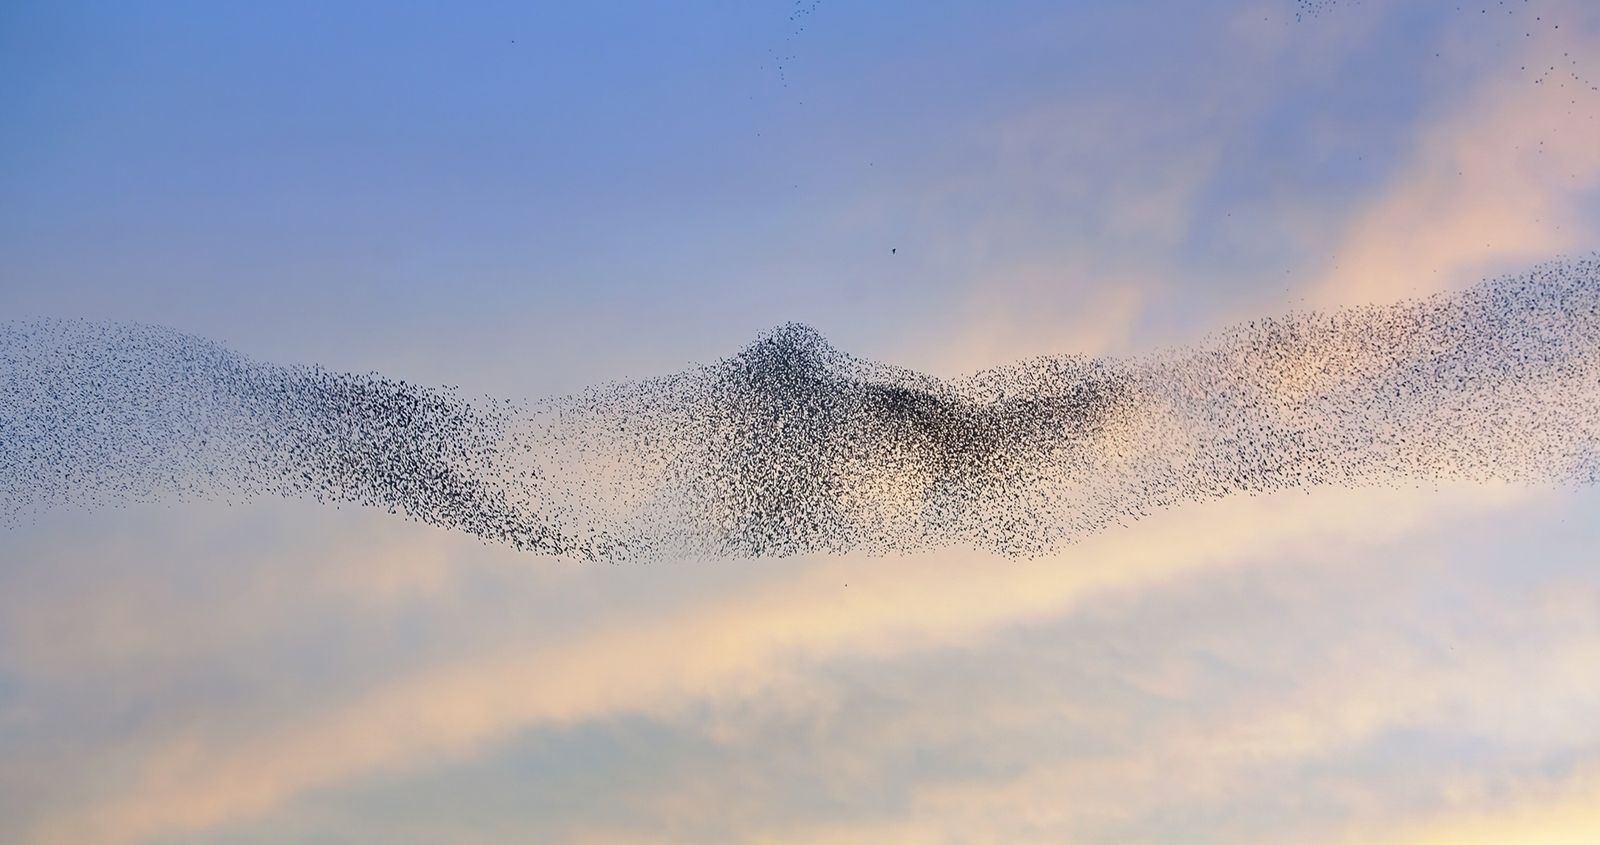
\includegraphics[height=0.62\textheight,keepaspectratio]{stara2.jpg}
    \end{column}
    \begin{column}{0.43\textwidth}
      \begin{itemize}
        \item Bandadas, cardúmenes, colonias bacterianas.
        \item Cada individuo decide sólo con sus vecinos.
        \item Del comportamiento local emerge orden global.
        \item \textbf{Materia activa:} la energía entra localmente, en cada agente.
      \end{itemize}
    \end{column}
  \end{columns}
\end{frame}

% ---------------------------------------------------------------- 4
\begin{frame}{Modelo matemático}
  \textbf{Vicsek (1995)} --- cada partícula adopta la dirección \emph{promedio} de sus vecinos:
  \[
    \theta_i(t+\Delta t) \;=\; \langle \theta(t)\rangle_{r_c} + \Delta\theta_i ,
    \qquad
    \langle\theta\rangle_{r_c} = \arctan\!\frac{\langle\sin\theta\rangle_{r_c}}{\langle\cos\theta\rangle_{r_c}}
  \]

  \textbf{Votante} --- cada partícula \emph{copia} a un vecino elegido al azar:
  \[
    \theta_i(t+\Delta t) \;=\; \theta_{j}(t) + \Delta\theta_i ,
    \qquad j \sim \mathcal{U}\{\,\text{vecinos de } i\,\}
  \]

  \textbf{Posición} --- común a ambos, rapidez constante:
  \[
    \vect{x}_i(t+\Delta t) = \vect{x}_i(t) + \vect{v}_i(t)\,\Delta t ,
    \qquad |\vect{v}_i| = v
  \]

  \vspace{0.3em}
  \centering
  Ruido angular uniforme: $\Delta\theta_i \in [-\eta/2,\; \eta/2]$

  \vspace{0.3em}
  {\footnotesize $\Delta t$, $v$ y $\eta$ son adimensionales (sin unidades físicas asociadas).}
\end{frame}

% =====================================================================
\section{Implementación}
% =====================================================================

% ---------------------------------------------------------------- 6
\begin{frame}{Arquitectura del motor}
  \begin{columns}[c]
    \begin{column}{0.60\textwidth}
      \centering
      \begin{tikzpicture}[
          scale=0.9, transform shape,
          font=\scriptsize,
          box/.style={draw=black!55, rounded corners=2pt, align=center,
                      inner xsep=6pt, inner ysep=5pt, text width=3.4cm},
          est/.style={box, fill=black!10},
          proc/.style={box, fill=white},
          dat/.style={box, fill=black!16},
          fl/.style={-{Latex[length=2mm]}, draw=black!60, thick}
        ]
        \node[est] (sim) {\texttt{Simulation}\\{\tiny estado: \texttt{particles\_}, \texttt{grid\_}, \texttt{rng\_}}};
        \node[proc, below=0.45cm of sim] (grid) {\texttt{Grid::rebuild()}\\{\tiny Cell Index Method}};
        \node[dat,  below=0.4cm of grid] (nl)  {\texttt{NeighborList}};
        \node[proc, below=0.4cm of nl] (rule) {\texttt{circularMeanHeading()}\\ \texttt{voterHeading()}\\{\tiny + \texttt{addAngularNoise()}}};
        \node[proc, below=0.4cm of rule] (int) {integración\\{\tiny posición + condiciones periódicas}};
        \draw[fl] (sim) -- (grid);
        \draw[fl] (grid) -- (nl);
        \draw[fl] (nl) -- (rule);
        \draw[fl] (rule) -- (int);
        \draw[fl] (int.east) -- ++(0.9,0) |- (sim.east);
      \end{tikzpicture}
    \end{column}
    \begin{column}{0.38\textwidth}
      \begin{itemize}
        \item Motor en \textbf{C\texttt{++}20}, sin dependencias externas.
        \item \texttt{Particle} guarda sólo $x$, $y$, $\theta$: la velocidad se deriva de $\theta$.
        \item Los dos modelos comparten todo salvo la regla de alineamiento.
      \end{itemize}
    \end{column}
  \end{columns}
\end{frame}

% ---------------------------------------------------------------- 7
\begin{frame}{Paso temporal: actualización sincrónica}
  \centering
  \begin{tikzpicture}[
      font=\small,
      node distance=0.55cm,
      pas/.style={draw=black!55, rounded corners=2pt, fill=black!5,
                  align=center, inner xsep=8pt, inner ysep=6pt, text width=3.2cm},
      fl/.style={-{Latex[length=2.4mm]}, draw=black!65, very thick}
    ]
    \node[pas] (p1) {\textbf{1. Vecinos}\\[2pt]{\scriptsize reconstruir la grilla desde las posiciones de $t$}};
    \node[pas, right=1.0cm of p1] (p2) {\textbf{2. Ángulos}\\[2pt]{\scriptsize calcular $\theta_i(t{+}\Delta t)$ leyendo \emph{sólo} el estado en $t$}};
    \node[pas, right=1.0cm of p2] (p3) {\textbf{3. Mover}\\[2pt]{\scriptsize avanzar con $\vect{v}_i(t)$ y recién ahí escribir $\theta_i(t{+}\Delta t)$}};
    \draw[fl] (p1) -- (p2);
    \draw[fl] (p2) -- (p3);
  \end{tikzpicture}

  \vspace{1.2em}
  \begin{itemize}
    \item Doble buffer en el paso 2: ninguna partícula ve el ángulo nuevo de otra dentro del mismo paso.
    \item Sin esa separación, el resultado dependería del orden de recorrido.
  \end{itemize}
\end{frame}

% =====================================================================
\section{Simulaciones}
% =====================================================================

% ---------------------------------------------------------------- 9
\begin{frame}{Sistema simulado}
  \begin{columns}[c]
    \begin{column}{0.44\textwidth}
      \centering
      \begin{tikzpicture}[scale=0.85, font=\scriptsize]
        \draw[black!70, thick] (0,0) rectangle (4.4,4.4);
        \foreach \x/\y/\a in {0.8/3.4/20, 1.4/3.0/35, 1.0/2.6/10,
                              3.3/1.2/200, 3.7/1.7/215, 3.0/0.7/190,
                              2.2/2.2/95, 0.6/1.0/300, 3.9/3.6/140}{
          \filldraw[black] (\x,\y) circle (1.4pt);
          \draw[-{Latex[length=1.6mm]}, thick] (\x,\y) -- ++(\a:0.55);
        }
        \draw[dashed, black!60] (2.2,2.2) circle (0.62);
        \node[black!60] at (2.95,2.75) {$r_c$};
        \draw[-{Latex[length=1.6mm]}, gray] (4.4,2.0) -- ++(0.45,0);
        \draw[-{Latex[length=1.6mm]}, gray] (-0.45,2.0) -- ++(0.45,0);
        \node[gray] at (2.2,-0.4) {condiciones periódicas de contorno};
        \draw[<->] (0,4.75) -- node[above] {$L = 10$} (4.4,4.75);
      \end{tikzpicture}
    \end{column}
    \begin{column}{0.54\textwidth}
      \params{
      \textbf{Parámetros fijos}\\[3pt]
      $L = 10$ \quad $r_c = 1$ \quad $\Delta t = 1$\\
      $v = 3\times10^{-2}$\\
      Condiciones periódicas de contorno.\\[8pt]
      \textbf{Input}\\[3pt]
      Ruido $\eta \in [0,\; 2\pi]$\\[8pt]
      \textbf{Densidades} \quad ($N = \rho L^2$)\\[3pt]
      $\rho \in [\,1/3\pi,\; 8\,]$ \quad ($N = 11$ a $800$)
      }
    \end{column}
  \end{columns}
\end{frame}

% ---------------------------------------------------------------- 10
\begin{frame}{Observables}
  \textbf{Polarización} --- módulo de la velocidad media, normalizado:
  \[
    v_a(t) \;=\; \frac{1}{N\,v}\;\Bigg|\sum_{k=1}^{N} \vect{v}_k(t)\Bigg|
    \;\in\; [0,\,1]
  \]

  \textbf{Fracción de la componente gigante} --- sobre el grafo de vecinos dentro de $r_c$:
  \[
    S(t) \;=\; \frac{N_{\max}(t)}{N},
    \qquad N_{\max} = \text{tamaño del cluster más grande}
  \]

  \vspace{0.4em}
  \hrule
  \vspace{0.5em}

  \params{
  Escalar reportado: media temporal en el estacionario.\\[3pt]
  Realizaciones: 10.\\[3pt]
  Pasos: $2\times10^{3}$ ($\rho = 2,\,4,\,8$), \; $1\times10^{4}$ ($\rho < 1$).\\[3pt]
  Ventana de promedio: desde el inicio del estacionario, medido por ruido.
  }
\end{frame}

% =====================================================================
\section{Resultados}
% =====================================================================

% ---------------------------------------------------------------- 12
\begin{frame}{Vicsek: dinámica característica}
  \begin{columns}[T]
    \begin{column}{0.36\textwidth}
      \animacion{frame_vicsek_rho2_ordenado.png}{1{,}0}{https://youtu.be/PENDIENTE-1}
    \end{column}
    \begin{column}{0.36\textwidth}
      \animacion{frame_vicsek_rho2_desordenado.png}{4{,}0}{https://youtu.be/PENDIENTE-2}
    \end{column}
    \begin{column}{0.26\textwidth}
      \params{$\rho = 2$ \ ($N = 200$)\\[6pt]Color según el ángulo de la velocidad.}
    \end{column}
  \end{columns}
\end{frame}

% ---------------------------------------------------------------- 13
\begin{frame}{Vicsek: evolución temporal de la polarización}
  \begin{columns}[c]
    \begin{column}{0.72\textwidth}
      \centering\includegraphics[width=0.98\linewidth,height=0.75\textheight,keepaspectratio]{va_t_vicsek_rho2.png}
    \end{column}
    \begin{column}{0.26\textwidth}
      \params{$\rho = 2$ \ ($N = 200$)}
    \end{column}
  \end{columns}
\end{frame}

% ---------------------------------------------------------------- 14
\begin{frame}{Vicsek: polarización en función del ruido}
  \begin{columns}[c]
    \begin{column}{0.72\textwidth}
      \centering\includegraphics[width=0.98\linewidth,height=0.75\textheight,keepaspectratio]{va_eta_vicsek.png}
    \end{column}
    \begin{column}{0.26\textwidth}
      \params{$2\times10^{3}$ pasos\\[6pt]Realizaciones: 10}
    \end{column}
  \end{columns}
\end{frame}

% ---------------------------------------------------------------- 15
\begin{frame}{Vicsek: evolución temporal de la componente gigante}
  \begin{columns}[c]
    \begin{column}{0.72\textwidth}
      \centering\includegraphics[width=0.98\linewidth,height=0.75\textheight,keepaspectratio]{S_t_vicsek_rho1_pi.png}
    \end{column}
    \begin{column}{0.26\textwidth}
      \params{$\rho = 1/\pi$ \ ($N = 32$)}
    \end{column}
  \end{columns}
\end{frame}

% ---------------------------------------------------------------- 16
\begin{frame}{Vicsek: componente gigante en función del ruido}
  \begin{columns}[c]
    \begin{column}{0.72\textwidth}
      \centering\includegraphics[width=0.98\linewidth,height=0.75\textheight,keepaspectratio]{S_eta_vicsek.png}
    \end{column}
    \begin{column}{0.26\textwidth}
      \params{$2\times10^{3}$ pasos ($\rho \geq 2$)\\$1\times10^{4}$ pasos ($\rho < 1$)\\[6pt]Realizaciones: 10}
    \end{column}
  \end{columns}
\end{frame}

% ---------------------------------------------------------------- 17
\begin{frame}{Votante: dinámica característica}
  \begin{columns}[T]
    \begin{column}{0.36\textwidth}
      \animacion{frame_voter_rho2_ordenado.png}{0{,}05}{https://youtu.be/PENDIENTE-3}
    \end{column}
    \begin{column}{0.36\textwidth}
      \animacion{frame_voter_rho2_desordenado.png}{1{,}0}{https://youtu.be/PENDIENTE-4}
    \end{column}
    \begin{column}{0.26\textwidth}
      \params{$\rho = 2$ \ ($N = 200$)\\[6pt]Color según el ángulo de la velocidad.}
    \end{column}
  \end{columns}
\end{frame}

% ---------------------------------------------------------------- 18
\begin{frame}{Votante: evolución temporal de la polarización}
  \begin{columns}[c]
    \begin{column}{0.72\textwidth}
      \centering\includegraphics[width=0.98\linewidth,height=0.75\textheight,keepaspectratio]{va_t_voter_rho2.png}
    \end{column}
    \begin{column}{0.26\textwidth}
      \params{$\rho = 2$ \ ($N = 200$)}
    \end{column}
  \end{columns}
\end{frame}

% ---------------------------------------------------------------- 19
\begin{frame}{Votante: polarización en función del ruido}
  \begin{columns}[c]
    \begin{column}{0.72\textwidth}
      \centering\includegraphics[width=0.98\linewidth,height=0.75\textheight,keepaspectratio]{va_eta_voter.png}
    \end{column}
    \begin{column}{0.26\textwidth}
      \params{$2\times10^{3}$ pasos\\[6pt]Realizaciones: 10}
    \end{column}
  \end{columns}
\end{frame}

% ---------------------------------------------------------------- 20
\begin{frame}{Votante: evolución temporal de la componente gigante}
  \begin{columns}[c]
    \begin{column}{0.72\textwidth}
      \centering\includegraphics[width=0.98\linewidth,height=0.75\textheight,keepaspectratio]{S_t_voter_rho1_pi.png}
    \end{column}
    \begin{column}{0.26\textwidth}
      \params{$\rho = 1/\pi$ \ ($N = 32$)}
    \end{column}
  \end{columns}
\end{frame}

% ---------------------------------------------------------------- 21
\begin{frame}{Votante: componente gigante en función del ruido}
  \begin{columns}[c]
    \begin{column}{0.72\textwidth}
      \centering\includegraphics[width=0.98\linewidth,height=0.75\textheight,keepaspectratio]{S_eta_voter.png}
    \end{column}
    \begin{column}{0.26\textwidth}
      \params{$2\times10^{3}$ pasos ($\rho \geq 2$)\\$1\times10^{4}$ pasos ($\rho < 1$)\\[6pt]Realizaciones: 10}
    \end{column}
  \end{columns}
\end{frame}

% ---------------------------------------------------------------- 22
\begin{frame}{Comparación: polarización}
  \begin{columns}[c]
    \begin{column}{0.72\textwidth}
      \centering\includegraphics[width=0.98\linewidth,height=0.75\textheight,keepaspectratio]{va_eta_comparacion_medias.png}
    \end{column}
    \begin{column}{0.26\textwidth}
      \params{Sólo el promedio\\[6pt]Realizaciones: 10}
    \end{column}
  \end{columns}
\end{frame}

% ---------------------------------------------------------------- 23
\begin{frame}{Comparación: componente gigante}
  \begin{columns}[c]
    \begin{column}{0.72\textwidth}
      \centering\includegraphics[width=0.98\linewidth,height=0.75\textheight,keepaspectratio]{S_eta_comparacion_sub_medias.png}
    \end{column}
    \begin{column}{0.26\textwidth}
      \params{$\rho = 1/\pi,\ 1/2\pi,\ 1/3\pi$\\$1\times10^{4}$ pasos\\[6pt]A $\rho = 2,\,4,\,8$ resulta $S \approx 1$ para todo $\eta$ en ambos modelos.}
    \end{column}
  \end{columns}
\end{frame}

% ---------------------------------------------------------------- 24
\begin{frame}{Polarización en función de la componente gigante}
  \begin{columns}[c]
    \begin{column}{0.84\textwidth}
      \centering\includegraphics[width=0.99\linewidth,height=0.66\textheight,keepaspectratio]{va_vs_S_paneles.png}
    \end{column}
    \begin{column}{0.15\textwidth}
      \params{Cada punto es un valor de $\eta$.}
    \end{column}
  \end{columns}
\end{frame}

% ---------------------------------------------------------------- 25
\begin{frame}{Tiempo de ejecución del Cell Index Method}
  \begin{columns}[c]
    \begin{column}{0.72\textwidth}
      \centering\includegraphics[width=0.98\linewidth,height=0.75\textheight,keepaspectratio]{benchmark_tp1_vs_tp2.png}
    \end{column}
    \begin{column}{0.26\textwidth}
      \params{
      $L = 10$, \ $r_c = 1$, \ $M = 9$\\
      Partículas puntuales\\[6pt]
      TP2: una medición por paso, $2\times10^{3}$ pasos\\[4pt]
      TP1: búsqueda aislada, repetida $2\times10^{2}$ veces
      }
    \end{column}
  \end{columns}
\end{frame}

% =====================================================================
\section{Conclusiones}
% =====================================================================

% ---------------------------------------------------------------- 27
\begin{frame}{Conclusiones}
  \begin{itemize}
    \item En ambos modelos $v_a$ decrece monótonamente con el ruido: hay transición de orden a desorden.
    \vspace{0.4em}
    \item En Vicsek el ruido tolerado \textbf{crece} con la densidad ($v_a = 0{,}5$ en $\eta = 2{,}9$, $3{,}2$ y $3{,}4$ para $\rho = 2$, $4$ y $8$).
    \vspace{0.4em}
    \item En el votante la dependencia se \textbf{invierte} ($\eta = 0{,}34$, $0{,}26$ y $0{,}21$) y la región ordenada es un orden de magnitud más angosta.
    \vspace{0.4em}
    \item $S \approx 1$ para $\rho = 2,\,4,\,8$ en todo el rango de $\eta$: la componente gigante sólo distingue regímenes en las densidades subcríticas.
    \vspace{0.4em}
    \item El CIM medido dentro del paso temporal tiene el mismo escalado con $N$ que medido aisladamente en el TP1.
  \end{itemize}
\end{frame}

% ---------------------------------------------------------------- 28
\begin{frame}[plain]
  \vfill
  \begin{beamercolorbox}[sep=8pt,center]{title}
    \usebeamerfont{title} Muchas gracias
  \end{beamercolorbox}
  \vfill
\end{frame}

\end{document}
"
%
%  La version "vivo" deja un hueco de color solido donde va cada animacion, que
%  presentacion/build_pptx.py detecta para pegar el GIF encima al armar el
%  .pptx (PowerPoint reproduce GIF animados en modo presentacion).
% =====================================================================
\documentclass[aspectratio=169]{beamer}

\usetheme{Boadilla}
\useoutertheme{miniframes}
\usecolortheme{whale}

\usepackage[utf8]{inputenc}
\usepackage[T1]{fontenc}
\usepackage[spanish,es-noquoting]{babel}
\usepackage{amsmath,amssymb,graphicx,booktabs}
\usepackage{tikz}
\usetikzlibrary{arrows.meta,positioning,fit,backgrounds,calc}

\graphicspath{{../data/plots/}{../data/plots/timeseries/}{../data/plots/eta/}{../data/plots/phase/}{../data/plots/benchmark/}{../data/plots/extra/}{./}{../informe/figs/}}

% Guia 3.5: vectores en negrita sin italica, escalares en italica sin negrita.
\newcommand{\vect}[1]{\mathbf{#1}}

\setbeamertemplate{navigation symbols}{}
\setbeamertemplate{footline}[frame number]
\setbeamercovered{transparent}

% Diapositiva divisoria automatica por seccion (guia 1.13). El color "title"
% de whale es texto blanco pensado para ir SOBRE la caja de fondo oscura que
% da beamercolorbox; usar solo el fg (como antes) deja texto blanco sobre el
% fondo blanco de la diapositiva -- invisible. beamercolorbox pinta ambos.
\AtBeginSection[]{%
  \begin{frame}[plain]
    \vfill
    \begin{beamercolorbox}[sep=8pt,center]{title}
      \usebeamerfont{title}\insertsection
    \end{beamercolorbox}
    \vfill
  \end{frame}
}

% Bloque de parametros al costado de una figura (guia 1.7). \footnotesize en
% vez de \scriptsize (guia 1.8: legible desde el fondo de la sala).
\newcommand{\params}[1]{{\footnotesize #1}}

% --- Modo de compilacion: entrega (default) vs. vivo ------------------
\providecommand{\modo}{entrega}
\def\modovivo{vivo}
% Color marcador del hueco de animacion. Se declara en RGB puro a proposito:
% build_pptx.py lo busca por valor exacto en la pagina rasterizada, y el
% "magenta" de xcolor se convierte a (236,0,139) al renderizar.
\definecolor{huecoanim}{RGB}{255,0,255}
\newcommand{\soloentrega}[1]{\ifx\modo\modovivo\else#1\fi}

% Una animacion: #1 fotograma, #2 valor de eta, #3 link.
% En modo "vivo" el fotograma se reemplaza por un cuadrado marcador -- la caja
% simulada es L x L y el GIF se renderiza cuadrado, asi que lo llena exacto --
% y el link no se imprime.
\newcommand{\animacion}[3]{%
  \centering
  \ifx\modo\modovivo
    \tikz\fill[huecoanim] (0,0) rectangle (0.48\textheight,0.48\textheight);%
  \else
    \includegraphics[height=0.48\textheight]{#1}%
  \fi
  \\[2pt]
  {\scriptsize $\eta = #2$}\\
  \soloentrega{{\tiny\color{blue}\url{#3}}}%
}

\title[Bandadas: Vicsek y Votante]{Autómata Off-Lattice: Bandadas de agentes autopropulsados}
\subtitle{Modelo de Vicsek y Modelo de Votante}
\author[Grupo 5]{Lucas Di Candia \and Juan Francisco Palermo \and Gonzalo Sharif Curi Martinez}
\institute[ITBA]{Grupo 5 --- Comisión S \\ Instituto Tecnológico de Buenos Aires}
\date{72.25 Simulación de Sistemas --- Trabajo Práctico N\textdegree{}2 --- 2026}

\begin{document}

% ---------------------------------------------------------------- 1
\begin{frame}[plain]
  \titlepage
\end{frame}

% =====================================================================
\section{Introducción}
% =====================================================================

% ---------------------------------------------------------------- 3
\begin{frame}{Sistema real}
  \begin{columns}[c]
    \begin{column}{0.55\textwidth}
      \centering
      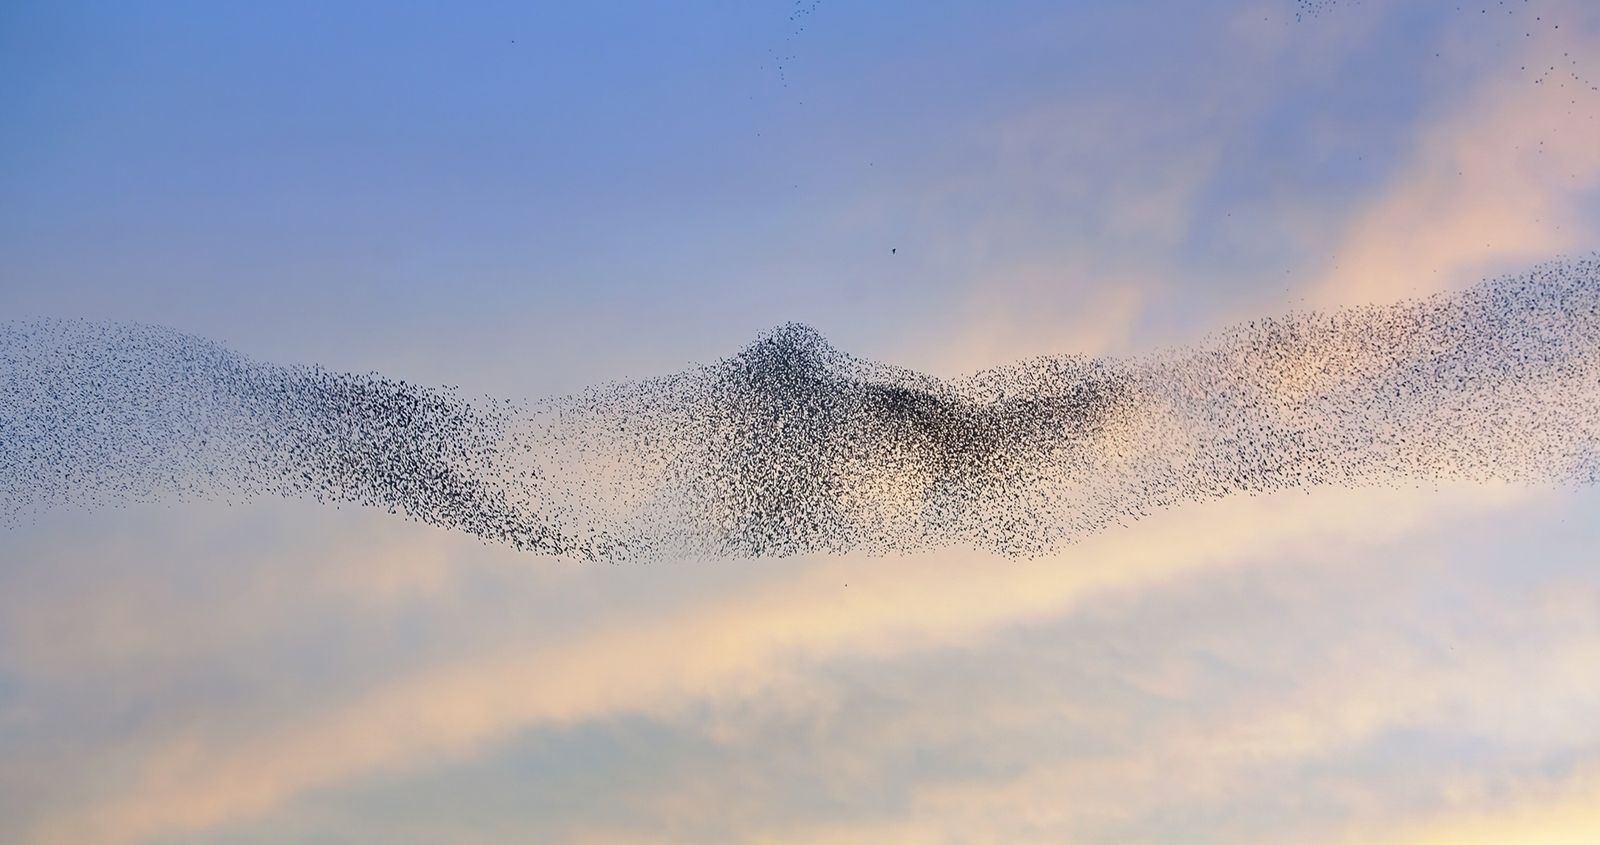
\includegraphics[height=0.62\textheight,keepaspectratio]{stara2.jpg}
    \end{column}
    \begin{column}{0.43\textwidth}
      \begin{itemize}
        \item Bandadas, cardúmenes, colonias bacterianas.
        \item Cada individuo decide sólo con sus vecinos.
        \item Del comportamiento local emerge orden global.
        \item \textbf{Materia activa:} la energía entra localmente, en cada agente.
      \end{itemize}
    \end{column}
  \end{columns}
\end{frame}

% ---------------------------------------------------------------- 4
\begin{frame}{Modelo matemático}
  \textbf{Vicsek (1995)} --- cada partícula adopta la dirección \emph{promedio} de sus vecinos:
  \[
    \theta_i(t+\Delta t) \;=\; \langle \theta(t)\rangle_{r_c} + \Delta\theta_i ,
    \qquad
    \langle\theta\rangle_{r_c} = \arctan\!\frac{\langle\sin\theta\rangle_{r_c}}{\langle\cos\theta\rangle_{r_c}}
  \]

  \textbf{Votante} --- cada partícula \emph{copia} a un vecino elegido al azar:
  \[
    \theta_i(t+\Delta t) \;=\; \theta_{j}(t) + \Delta\theta_i ,
    \qquad j \sim \mathcal{U}\{\,\text{vecinos de } i\,\}
  \]

  \textbf{Posición} --- común a ambos, rapidez constante:
  \[
    \vect{x}_i(t+\Delta t) = \vect{x}_i(t) + \vect{v}_i(t)\,\Delta t ,
    \qquad |\vect{v}_i| = v
  \]

  \vspace{0.3em}
  \centering
  Ruido angular uniforme: $\Delta\theta_i \in [-\eta/2,\; \eta/2]$

  \vspace{0.3em}
  {\footnotesize $\Delta t$, $v$ y $\eta$ son adimensionales (sin unidades físicas asociadas).}
\end{frame}

% =====================================================================
\section{Implementación}
% =====================================================================

% ---------------------------------------------------------------- 6
\begin{frame}{Arquitectura del motor}
  \begin{columns}[c]
    \begin{column}{0.60\textwidth}
      \centering
      \begin{tikzpicture}[
          scale=0.9, transform shape,
          font=\scriptsize,
          box/.style={draw=black!55, rounded corners=2pt, align=center,
                      inner xsep=6pt, inner ysep=5pt, text width=3.4cm},
          est/.style={box, fill=black!10},
          proc/.style={box, fill=white},
          dat/.style={box, fill=black!16},
          fl/.style={-{Latex[length=2mm]}, draw=black!60, thick}
        ]
        \node[est] (sim) {\texttt{Simulation}\\{\tiny estado: \texttt{particles\_}, \texttt{grid\_}, \texttt{rng\_}}};
        \node[proc, below=0.45cm of sim] (grid) {\texttt{Grid::rebuild()}\\{\tiny Cell Index Method}};
        \node[dat,  below=0.4cm of grid] (nl)  {\texttt{NeighborList}};
        \node[proc, below=0.4cm of nl] (rule) {\texttt{circularMeanHeading()}\\ \texttt{voterHeading()}\\{\tiny + \texttt{addAngularNoise()}}};
        \node[proc, below=0.4cm of rule] (int) {integración\\{\tiny posición + condiciones periódicas}};
        \draw[fl] (sim) -- (grid);
        \draw[fl] (grid) -- (nl);
        \draw[fl] (nl) -- (rule);
        \draw[fl] (rule) -- (int);
        \draw[fl] (int.east) -- ++(0.9,0) |- (sim.east);
      \end{tikzpicture}
    \end{column}
    \begin{column}{0.38\textwidth}
      \begin{itemize}
        \item Motor en \textbf{C\texttt{++}20}, sin dependencias externas.
        \item \texttt{Particle} guarda sólo $x$, $y$, $\theta$: la velocidad se deriva de $\theta$.
        \item Los dos modelos comparten todo salvo la regla de alineamiento.
      \end{itemize}
    \end{column}
  \end{columns}
\end{frame}

% ---------------------------------------------------------------- 7
\begin{frame}{Paso temporal: actualización sincrónica}
  \centering
  \begin{tikzpicture}[
      font=\small,
      node distance=0.55cm,
      pas/.style={draw=black!55, rounded corners=2pt, fill=black!5,
                  align=center, inner xsep=8pt, inner ysep=6pt, text width=3.2cm},
      fl/.style={-{Latex[length=2.4mm]}, draw=black!65, very thick}
    ]
    \node[pas] (p1) {\textbf{1. Vecinos}\\[2pt]{\scriptsize reconstruir la grilla desde las posiciones de $t$}};
    \node[pas, right=1.0cm of p1] (p2) {\textbf{2. Ángulos}\\[2pt]{\scriptsize calcular $\theta_i(t{+}\Delta t)$ leyendo \emph{sólo} el estado en $t$}};
    \node[pas, right=1.0cm of p2] (p3) {\textbf{3. Mover}\\[2pt]{\scriptsize avanzar con $\vect{v}_i(t)$ y recién ahí escribir $\theta_i(t{+}\Delta t)$}};
    \draw[fl] (p1) -- (p2);
    \draw[fl] (p2) -- (p3);
  \end{tikzpicture}

  \vspace{1.2em}
  \begin{itemize}
    \item Doble buffer en el paso 2: ninguna partícula ve el ángulo nuevo de otra dentro del mismo paso.
    \item Sin esa separación, el resultado dependería del orden de recorrido.
  \end{itemize}
\end{frame}

% =====================================================================
\section{Simulaciones}
% =====================================================================

% ---------------------------------------------------------------- 9
\begin{frame}{Sistema simulado}
  \begin{columns}[c]
    \begin{column}{0.44\textwidth}
      \centering
      \begin{tikzpicture}[scale=0.85, font=\scriptsize]
        \draw[black!70, thick] (0,0) rectangle (4.4,4.4);
        \foreach \x/\y/\a in {0.8/3.4/20, 1.4/3.0/35, 1.0/2.6/10,
                              3.3/1.2/200, 3.7/1.7/215, 3.0/0.7/190,
                              2.2/2.2/95, 0.6/1.0/300, 3.9/3.6/140}{
          \filldraw[black] (\x,\y) circle (1.4pt);
          \draw[-{Latex[length=1.6mm]}, thick] (\x,\y) -- ++(\a:0.55);
        }
        \draw[dashed, black!60] (2.2,2.2) circle (0.62);
        \node[black!60] at (2.95,2.75) {$r_c$};
        \draw[-{Latex[length=1.6mm]}, gray] (4.4,2.0) -- ++(0.45,0);
        \draw[-{Latex[length=1.6mm]}, gray] (-0.45,2.0) -- ++(0.45,0);
        \node[gray] at (2.2,-0.4) {condiciones periódicas de contorno};
        \draw[<->] (0,4.75) -- node[above] {$L = 10$} (4.4,4.75);
      \end{tikzpicture}
    \end{column}
    \begin{column}{0.54\textwidth}
      \params{
      \textbf{Parámetros fijos}\\[3pt]
      $L = 10$ \quad $r_c = 1$ \quad $\Delta t = 1$\\
      $v = 3\times10^{-2}$\\
      Condiciones periódicas de contorno.\\[8pt]
      \textbf{Input}\\[3pt]
      Ruido $\eta \in [0,\; 2\pi]$\\[8pt]
      \textbf{Densidades} \quad ($N = \rho L^2$)\\[3pt]
      $\rho \in [\,1/3\pi,\; 8\,]$ \quad ($N = 11$ a $800$)
      }
    \end{column}
  \end{columns}
\end{frame}

% ---------------------------------------------------------------- 10
\begin{frame}{Observables}
  \textbf{Polarización} --- módulo de la velocidad media, normalizado:
  \[
    v_a(t) \;=\; \frac{1}{N\,v}\;\Bigg|\sum_{k=1}^{N} \vect{v}_k(t)\Bigg|
    \;\in\; [0,\,1]
  \]

  \textbf{Fracción de la componente gigante} --- sobre el grafo de vecinos dentro de $r_c$:
  \[
    S(t) \;=\; \frac{N_{\max}(t)}{N},
    \qquad N_{\max} = \text{tamaño del cluster más grande}
  \]

  \vspace{0.4em}
  \hrule
  \vspace{0.5em}

  \params{
  Escalar reportado: media temporal en el estacionario.\\[3pt]
  Realizaciones: 10.\\[3pt]
  Pasos: $2\times10^{3}$ ($\rho = 2,\,4,\,8$), \; $1\times10^{4}$ ($\rho < 1$).\\[3pt]
  Ventana de promedio: desde el inicio del estacionario, medido por ruido.
  }
\end{frame}

% =====================================================================
\section{Resultados}
% =====================================================================

% ---------------------------------------------------------------- 12
\begin{frame}{Vicsek: dinámica característica}
  \begin{columns}[T]
    \begin{column}{0.36\textwidth}
      \animacion{frame_vicsek_rho2_ordenado.png}{1{,}0}{https://youtu.be/PENDIENTE-1}
    \end{column}
    \begin{column}{0.36\textwidth}
      \animacion{frame_vicsek_rho2_desordenado.png}{4{,}0}{https://youtu.be/PENDIENTE-2}
    \end{column}
    \begin{column}{0.26\textwidth}
      \params{$\rho = 2$ \ ($N = 200$)\\[6pt]Color según el ángulo de la velocidad.}
    \end{column}
  \end{columns}
\end{frame}

% ---------------------------------------------------------------- 13
\begin{frame}{Vicsek: evolución temporal de la polarización}
  \begin{columns}[c]
    \begin{column}{0.72\textwidth}
      \centering\includegraphics[width=0.98\linewidth,height=0.75\textheight,keepaspectratio]{va_t_vicsek_rho2.png}
    \end{column}
    \begin{column}{0.26\textwidth}
      \params{$\rho = 2$ \ ($N = 200$)}
    \end{column}
  \end{columns}
\end{frame}

% ---------------------------------------------------------------- 14
\begin{frame}{Vicsek: polarización en función del ruido}
  \begin{columns}[c]
    \begin{column}{0.72\textwidth}
      \centering\includegraphics[width=0.98\linewidth,height=0.75\textheight,keepaspectratio]{va_eta_vicsek.png}
    \end{column}
    \begin{column}{0.26\textwidth}
      \params{$2\times10^{3}$ pasos\\[6pt]Realizaciones: 10}
    \end{column}
  \end{columns}
\end{frame}

% ---------------------------------------------------------------- 15
\begin{frame}{Vicsek: evolución temporal de la componente gigante}
  \begin{columns}[c]
    \begin{column}{0.72\textwidth}
      \centering\includegraphics[width=0.98\linewidth,height=0.75\textheight,keepaspectratio]{S_t_vicsek_rho1_pi.png}
    \end{column}
    \begin{column}{0.26\textwidth}
      \params{$\rho = 1/\pi$ \ ($N = 32$)}
    \end{column}
  \end{columns}
\end{frame}

% ---------------------------------------------------------------- 16
\begin{frame}{Vicsek: componente gigante en función del ruido}
  \begin{columns}[c]
    \begin{column}{0.72\textwidth}
      \centering\includegraphics[width=0.98\linewidth,height=0.75\textheight,keepaspectratio]{S_eta_vicsek.png}
    \end{column}
    \begin{column}{0.26\textwidth}
      \params{$2\times10^{3}$ pasos ($\rho \geq 2$)\\$1\times10^{4}$ pasos ($\rho < 1$)\\[6pt]Realizaciones: 10}
    \end{column}
  \end{columns}
\end{frame}

% ---------------------------------------------------------------- 17
\begin{frame}{Votante: dinámica característica}
  \begin{columns}[T]
    \begin{column}{0.36\textwidth}
      \animacion{frame_voter_rho2_ordenado.png}{0{,}05}{https://youtu.be/PENDIENTE-3}
    \end{column}
    \begin{column}{0.36\textwidth}
      \animacion{frame_voter_rho2_desordenado.png}{1{,}0}{https://youtu.be/PENDIENTE-4}
    \end{column}
    \begin{column}{0.26\textwidth}
      \params{$\rho = 2$ \ ($N = 200$)\\[6pt]Color según el ángulo de la velocidad.}
    \end{column}
  \end{columns}
\end{frame}

% ---------------------------------------------------------------- 18
\begin{frame}{Votante: evolución temporal de la polarización}
  \begin{columns}[c]
    \begin{column}{0.72\textwidth}
      \centering\includegraphics[width=0.98\linewidth,height=0.75\textheight,keepaspectratio]{va_t_voter_rho2.png}
    \end{column}
    \begin{column}{0.26\textwidth}
      \params{$\rho = 2$ \ ($N = 200$)}
    \end{column}
  \end{columns}
\end{frame}

% ---------------------------------------------------------------- 19
\begin{frame}{Votante: polarización en función del ruido}
  \begin{columns}[c]
    \begin{column}{0.72\textwidth}
      \centering\includegraphics[width=0.98\linewidth,height=0.75\textheight,keepaspectratio]{va_eta_voter.png}
    \end{column}
    \begin{column}{0.26\textwidth}
      \params{$2\times10^{3}$ pasos\\[6pt]Realizaciones: 10}
    \end{column}
  \end{columns}
\end{frame}

% ---------------------------------------------------------------- 20
\begin{frame}{Votante: evolución temporal de la componente gigante}
  \begin{columns}[c]
    \begin{column}{0.72\textwidth}
      \centering\includegraphics[width=0.98\linewidth,height=0.75\textheight,keepaspectratio]{S_t_voter_rho1_pi.png}
    \end{column}
    \begin{column}{0.26\textwidth}
      \params{$\rho = 1/\pi$ \ ($N = 32$)}
    \end{column}
  \end{columns}
\end{frame}

% ---------------------------------------------------------------- 21
\begin{frame}{Votante: componente gigante en función del ruido}
  \begin{columns}[c]
    \begin{column}{0.72\textwidth}
      \centering\includegraphics[width=0.98\linewidth,height=0.75\textheight,keepaspectratio]{S_eta_voter.png}
    \end{column}
    \begin{column}{0.26\textwidth}
      \params{$2\times10^{3}$ pasos ($\rho \geq 2$)\\$1\times10^{4}$ pasos ($\rho < 1$)\\[6pt]Realizaciones: 10}
    \end{column}
  \end{columns}
\end{frame}

% ---------------------------------------------------------------- 22
\begin{frame}{Comparación: polarización}
  \begin{columns}[c]
    \begin{column}{0.72\textwidth}
      \centering\includegraphics[width=0.98\linewidth,height=0.75\textheight,keepaspectratio]{va_eta_comparacion_medias.png}
    \end{column}
    \begin{column}{0.26\textwidth}
      \params{Sólo el promedio\\[6pt]Realizaciones: 10}
    \end{column}
  \end{columns}
\end{frame}

% ---------------------------------------------------------------- 23
\begin{frame}{Comparación: componente gigante}
  \begin{columns}[c]
    \begin{column}{0.72\textwidth}
      \centering\includegraphics[width=0.98\linewidth,height=0.75\textheight,keepaspectratio]{S_eta_comparacion_sub_medias.png}
    \end{column}
    \begin{column}{0.26\textwidth}
      \params{$\rho = 1/\pi,\ 1/2\pi,\ 1/3\pi$\\$1\times10^{4}$ pasos\\[6pt]A $\rho = 2,\,4,\,8$ resulta $S \approx 1$ para todo $\eta$ en ambos modelos.}
    \end{column}
  \end{columns}
\end{frame}

% ---------------------------------------------------------------- 24
\begin{frame}{Polarización en función de la componente gigante}
  \begin{columns}[c]
    \begin{column}{0.84\textwidth}
      \centering\includegraphics[width=0.99\linewidth,height=0.66\textheight,keepaspectratio]{va_vs_S_paneles.png}
    \end{column}
    \begin{column}{0.15\textwidth}
      \params{Cada punto es un valor de $\eta$.}
    \end{column}
  \end{columns}
\end{frame}

% ---------------------------------------------------------------- 25
\begin{frame}{Tiempo de ejecución del Cell Index Method}
  \begin{columns}[c]
    \begin{column}{0.72\textwidth}
      \centering\includegraphics[width=0.98\linewidth,height=0.75\textheight,keepaspectratio]{benchmark_tp1_vs_tp2.png}
    \end{column}
    \begin{column}{0.26\textwidth}
      \params{
      $L = 10$, \ $r_c = 1$, \ $M = 9$\\
      Partículas puntuales\\[6pt]
      TP2: una medición por paso, $2\times10^{3}$ pasos\\[4pt]
      TP1: búsqueda aislada, repetida $2\times10^{2}$ veces
      }
    \end{column}
  \end{columns}
\end{frame}

% =====================================================================
\section{Conclusiones}
% =====================================================================

% ---------------------------------------------------------------- 27
\begin{frame}{Conclusiones}
  \begin{itemize}
    \item En ambos modelos $v_a$ decrece monótonamente con el ruido: hay transición de orden a desorden.
    \vspace{0.4em}
    \item En Vicsek el ruido tolerado \textbf{crece} con la densidad ($v_a = 0{,}5$ en $\eta = 2{,}9$, $3{,}2$ y $3{,}4$ para $\rho = 2$, $4$ y $8$).
    \vspace{0.4em}
    \item En el votante la dependencia se \textbf{invierte} ($\eta = 0{,}34$, $0{,}26$ y $0{,}21$) y la región ordenada es un orden de magnitud más angosta.
    \vspace{0.4em}
    \item $S \approx 1$ para $\rho = 2,\,4,\,8$ en todo el rango de $\eta$: la componente gigante sólo distingue regímenes en las densidades subcríticas.
    \vspace{0.4em}
    \item El CIM medido dentro del paso temporal tiene el mismo escalado con $N$ que medido aisladamente en el TP1.
  \end{itemize}
\end{frame}

% ---------------------------------------------------------------- 28
\begin{frame}[plain]
  \vfill
  \begin{beamercolorbox}[sep=8pt,center]{title}
    \usebeamerfont{title} Muchas gracias
  \end{beamercolorbox}
  \vfill
\end{frame}

\end{document}
"
%
%  La version "vivo" deja un hueco de color solido donde va cada animacion, que
%  presentacion/build_pptx.py detecta para pegar el GIF encima al armar el
%  .pptx (PowerPoint reproduce GIF animados en modo presentacion).
% =====================================================================
\documentclass[aspectratio=169]{beamer}

\usetheme{Boadilla}
\useoutertheme{miniframes}
\usecolortheme{whale}

\usepackage[utf8]{inputenc}
\usepackage[T1]{fontenc}
\usepackage[spanish,es-noquoting]{babel}
\usepackage{amsmath,amssymb,graphicx,booktabs}
\usepackage{tikz}
\usetikzlibrary{arrows.meta,positioning,fit,backgrounds,calc}

\graphicspath{{../data/plots/}{../data/plots/timeseries/}{../data/plots/eta/}{../data/plots/phase/}{../data/plots/benchmark/}{../data/plots/extra/}{./}{../informe/figs/}}

% Guia 3.5: vectores en negrita sin italica, escalares en italica sin negrita.
\newcommand{\vect}[1]{\mathbf{#1}}

\setbeamertemplate{navigation symbols}{}
\setbeamertemplate{footline}[frame number]
\setbeamercovered{transparent}

% Diapositiva divisoria automatica por seccion (guia 1.13). El color "title"
% de whale es texto blanco pensado para ir SOBRE la caja de fondo oscura que
% da beamercolorbox; usar solo el fg (como antes) deja texto blanco sobre el
% fondo blanco de la diapositiva -- invisible. beamercolorbox pinta ambos.
\AtBeginSection[]{%
  \begin{frame}[plain]
    \vfill
    \begin{beamercolorbox}[sep=8pt,center]{title}
      \usebeamerfont{title}\insertsection
    \end{beamercolorbox}
    \vfill
  \end{frame}
}

% Bloque de parametros al costado de una figura (guia 1.7). \footnotesize en
% vez de \scriptsize (guia 1.8: legible desde el fondo de la sala).
\newcommand{\params}[1]{{\footnotesize #1}}

% --- Modo de compilacion: entrega (default) vs. vivo ------------------
\providecommand{\modo}{entrega}
\def\modovivo{vivo}
% Color marcador del hueco de animacion. Se declara en RGB puro a proposito:
% build_pptx.py lo busca por valor exacto en la pagina rasterizada, y el
% "magenta" de xcolor se convierte a (236,0,139) al renderizar.
\definecolor{huecoanim}{RGB}{255,0,255}
\newcommand{\soloentrega}[1]{\ifx\modo\modovivo\else#1\fi}

% Una animacion: #1 fotograma, #2 valor de eta, #3 link.
% En modo "vivo" el fotograma se reemplaza por un cuadrado marcador -- la caja
% simulada es L x L y el GIF se renderiza cuadrado, asi que lo llena exacto --
% y el link no se imprime.
\newcommand{\animacion}[3]{%
  \centering
  \ifx\modo\modovivo
    \tikz\fill[huecoanim] (0,0) rectangle (0.48\textheight,0.48\textheight);%
  \else
    \includegraphics[height=0.48\textheight]{#1}%
  \fi
  \\[2pt]
  {\scriptsize $\eta = #2$}\\
  \soloentrega{{\tiny\color{blue}\url{#3}}}%
}

\title[Bandadas: Vicsek y Votante]{Autómata Off-Lattice: Bandadas de agentes autopropulsados}
\subtitle{Modelo de Vicsek y Modelo de Votante}
\author[Grupo 5]{Lucas Di Candia \and Juan Francisco Palermo \and Gonzalo Sharif Curi Martinez}
\institute[ITBA]{Grupo 5 --- Comisión S \\ Instituto Tecnológico de Buenos Aires}
\date{72.25 Simulación de Sistemas --- Trabajo Práctico N\textdegree{}2 --- 2026}

\begin{document}

% ---------------------------------------------------------------- 1
\begin{frame}[plain]
  \titlepage
\end{frame}

% =====================================================================
\section{Introducción}
% =====================================================================

% ---------------------------------------------------------------- 3
\begin{frame}{Sistema real}
  \begin{columns}[c]
    \begin{column}{0.55\textwidth}
      \centering
      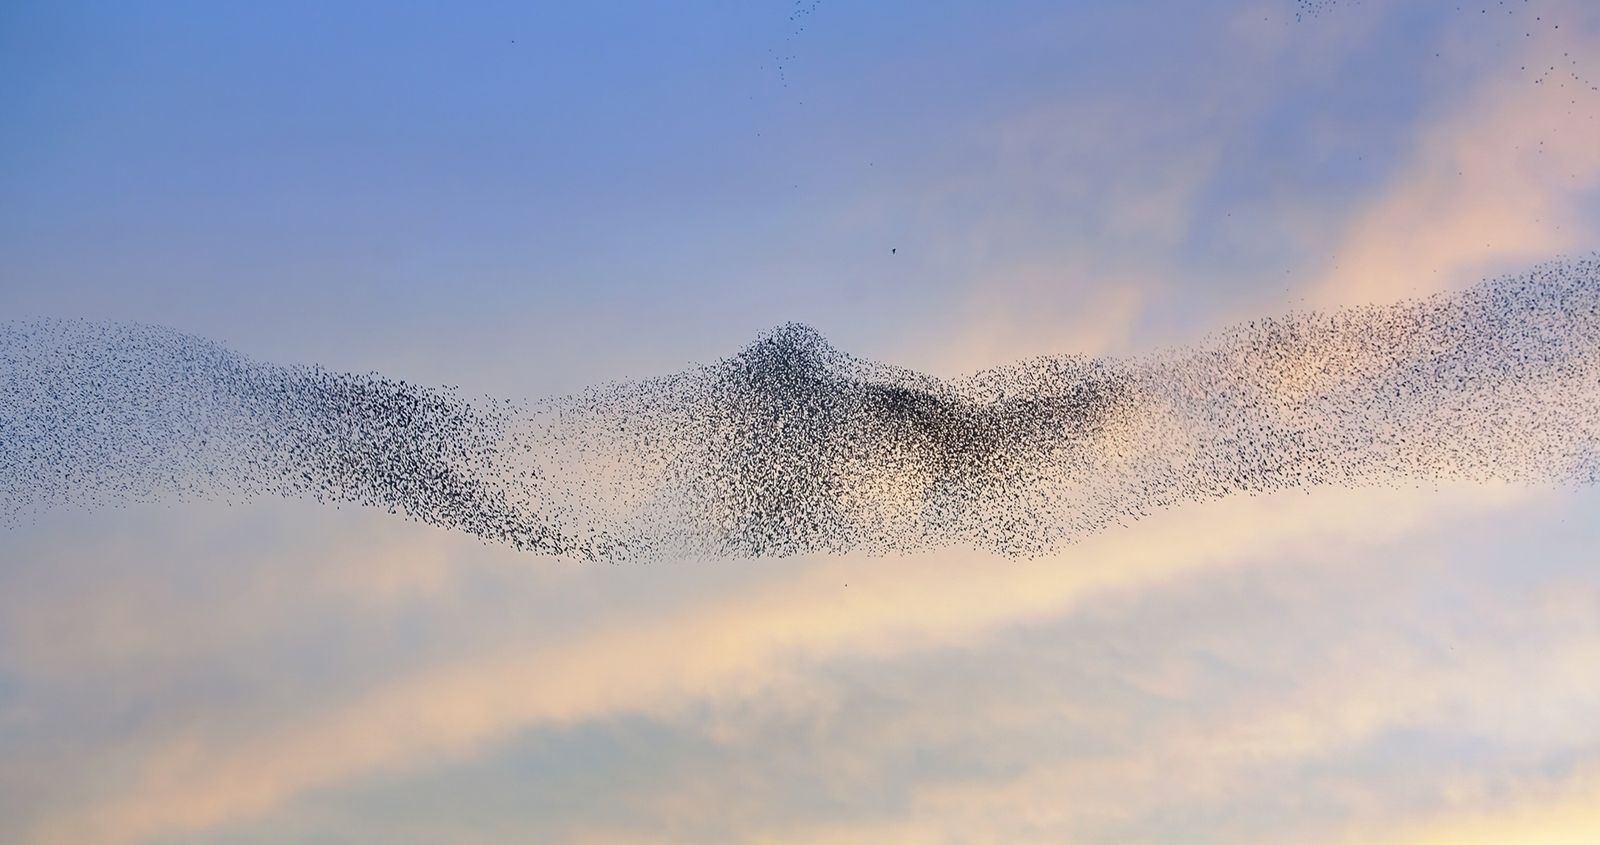
\includegraphics[height=0.62\textheight,keepaspectratio]{stara2.jpg}
    \end{column}
    \begin{column}{0.43\textwidth}
      \begin{itemize}
        \item Bandadas, cardúmenes, colonias bacterianas.
        \item Cada individuo decide sólo con sus vecinos.
        \item Del comportamiento local emerge orden global.
        \item \textbf{Materia activa:} la energía entra localmente, en cada agente.
      \end{itemize}
    \end{column}
  \end{columns}
\end{frame}

% ---------------------------------------------------------------- 4
\begin{frame}{Modelo matemático}
  \textbf{Vicsek (1995)} --- cada partícula adopta la dirección \emph{promedio} de sus vecinos:
  \[
    \theta_i(t+\Delta t) \;=\; \langle \theta(t)\rangle_{r_c} + \Delta\theta_i ,
    \qquad
    \langle\theta\rangle_{r_c} = \arctan\!\frac{\langle\sin\theta\rangle_{r_c}}{\langle\cos\theta\rangle_{r_c}}
  \]

  \textbf{Votante} --- cada partícula \emph{copia} a un vecino elegido al azar:
  \[
    \theta_i(t+\Delta t) \;=\; \theta_{j}(t) + \Delta\theta_i ,
    \qquad j \sim \mathcal{U}\{\,\text{vecinos de } i\,\}
  \]

  \textbf{Posición} --- común a ambos, rapidez constante:
  \[
    \vect{x}_i(t+\Delta t) = \vect{x}_i(t) + \vect{v}_i(t)\,\Delta t ,
    \qquad |\vect{v}_i| = v
  \]

  \vspace{0.3em}
  \centering
  Ruido angular uniforme: $\Delta\theta_i \in [-\eta/2,\; \eta/2]$

  \vspace{0.3em}
  {\footnotesize $\Delta t$, $v$ y $\eta$ son adimensionales (sin unidades físicas asociadas).}
\end{frame}

% =====================================================================
\section{Implementación}
% =====================================================================

% ---------------------------------------------------------------- 6
\begin{frame}{Arquitectura del motor}
  \begin{columns}[c]
    \begin{column}{0.60\textwidth}
      \centering
      \begin{tikzpicture}[
          scale=0.9, transform shape,
          font=\scriptsize,
          box/.style={draw=black!55, rounded corners=2pt, align=center,
                      inner xsep=6pt, inner ysep=5pt, text width=3.4cm},
          est/.style={box, fill=black!10},
          proc/.style={box, fill=white},
          dat/.style={box, fill=black!16},
          fl/.style={-{Latex[length=2mm]}, draw=black!60, thick}
        ]
        \node[est] (sim) {\texttt{Simulation}\\{\tiny estado: \texttt{particles\_}, \texttt{grid\_}, \texttt{rng\_}}};
        \node[proc, below=0.45cm of sim] (grid) {\texttt{Grid::rebuild()}\\{\tiny Cell Index Method}};
        \node[dat,  below=0.4cm of grid] (nl)  {\texttt{NeighborList}};
        \node[proc, below=0.4cm of nl] (rule) {\texttt{circularMeanHeading()}\\ \texttt{voterHeading()}\\{\tiny + \texttt{addAngularNoise()}}};
        \node[proc, below=0.4cm of rule] (int) {integración\\{\tiny posición + condiciones periódicas}};
        \draw[fl] (sim) -- (grid);
        \draw[fl] (grid) -- (nl);
        \draw[fl] (nl) -- (rule);
        \draw[fl] (rule) -- (int);
        \draw[fl] (int.east) -- ++(0.9,0) |- (sim.east);
      \end{tikzpicture}
    \end{column}
    \begin{column}{0.38\textwidth}
      \begin{itemize}
        \item Motor en \textbf{C\texttt{++}20}, sin dependencias externas.
        \item \texttt{Particle} guarda sólo $x$, $y$, $\theta$: la velocidad se deriva de $\theta$.
        \item Los dos modelos comparten todo salvo la regla de alineamiento.
      \end{itemize}
    \end{column}
  \end{columns}
\end{frame}

% ---------------------------------------------------------------- 7
\begin{frame}{Paso temporal: actualización sincrónica}
  \centering
  \begin{tikzpicture}[
      font=\small,
      node distance=0.55cm,
      pas/.style={draw=black!55, rounded corners=2pt, fill=black!5,
                  align=center, inner xsep=8pt, inner ysep=6pt, text width=3.2cm},
      fl/.style={-{Latex[length=2.4mm]}, draw=black!65, very thick}
    ]
    \node[pas] (p1) {\textbf{1. Vecinos}\\[2pt]{\scriptsize reconstruir la grilla desde las posiciones de $t$}};
    \node[pas, right=1.0cm of p1] (p2) {\textbf{2. Ángulos}\\[2pt]{\scriptsize calcular $\theta_i(t{+}\Delta t)$ leyendo \emph{sólo} el estado en $t$}};
    \node[pas, right=1.0cm of p2] (p3) {\textbf{3. Mover}\\[2pt]{\scriptsize avanzar con $\vect{v}_i(t)$ y recién ahí escribir $\theta_i(t{+}\Delta t)$}};
    \draw[fl] (p1) -- (p2);
    \draw[fl] (p2) -- (p3);
  \end{tikzpicture}

  \vspace{1.2em}
  \begin{itemize}
    \item Doble buffer en el paso 2: ninguna partícula ve el ángulo nuevo de otra dentro del mismo paso.
    \item Sin esa separación, el resultado dependería del orden de recorrido.
  \end{itemize}
\end{frame}

% =====================================================================
\section{Simulaciones}
% =====================================================================

% ---------------------------------------------------------------- 9
\begin{frame}{Sistema simulado}
  \begin{columns}[c]
    \begin{column}{0.44\textwidth}
      \centering
      \begin{tikzpicture}[scale=0.85, font=\scriptsize]
        \draw[black!70, thick] (0,0) rectangle (4.4,4.4);
        \foreach \x/\y/\a in {0.8/3.4/20, 1.4/3.0/35, 1.0/2.6/10,
                              3.3/1.2/200, 3.7/1.7/215, 3.0/0.7/190,
                              2.2/2.2/95, 0.6/1.0/300, 3.9/3.6/140}{
          \filldraw[black] (\x,\y) circle (1.4pt);
          \draw[-{Latex[length=1.6mm]}, thick] (\x,\y) -- ++(\a:0.55);
        }
        \draw[dashed, black!60] (2.2,2.2) circle (0.62);
        \node[black!60] at (2.95,2.75) {$r_c$};
        \draw[-{Latex[length=1.6mm]}, gray] (4.4,2.0) -- ++(0.45,0);
        \draw[-{Latex[length=1.6mm]}, gray] (-0.45,2.0) -- ++(0.45,0);
        \node[gray] at (2.2,-0.4) {condiciones periódicas de contorno};
        \draw[<->] (0,4.75) -- node[above] {$L = 10$} (4.4,4.75);
      \end{tikzpicture}
    \end{column}
    \begin{column}{0.54\textwidth}
      \params{
      \textbf{Parámetros fijos}\\[3pt]
      $L = 10$ \quad $r_c = 1$ \quad $\Delta t = 1$\\
      $v = 3\times10^{-2}$\\
      Condiciones periódicas de contorno.\\[8pt]
      \textbf{Input}\\[3pt]
      Ruido $\eta \in [0,\; 2\pi]$\\[8pt]
      \textbf{Densidades} \quad ($N = \rho L^2$)\\[3pt]
      $\rho \in [\,1/3\pi,\; 8\,]$ \quad ($N = 11$ a $800$)
      }
    \end{column}
  \end{columns}
\end{frame}

% ---------------------------------------------------------------- 10
\begin{frame}{Observables}
  \textbf{Polarización} --- módulo de la velocidad media, normalizado:
  \[
    v_a(t) \;=\; \frac{1}{N\,v}\;\Bigg|\sum_{k=1}^{N} \vect{v}_k(t)\Bigg|
    \;\in\; [0,\,1]
  \]

  \textbf{Fracción de la componente gigante} --- sobre el grafo de vecinos dentro de $r_c$:
  \[
    S(t) \;=\; \frac{N_{\max}(t)}{N},
    \qquad N_{\max} = \text{tamaño del cluster más grande}
  \]

  \vspace{0.4em}
  \hrule
  \vspace{0.5em}

  \params{
  Escalar reportado: media temporal en el estacionario.\\[3pt]
  Realizaciones: 10.\\[3pt]
  Pasos: $2\times10^{3}$ ($\rho = 2,\,4,\,8$), \; $1\times10^{4}$ ($\rho < 1$).\\[3pt]
  Ventana de promedio: desde el inicio del estacionario, medido por ruido.
  }
\end{frame}

% =====================================================================
\section{Resultados}
% =====================================================================

% ---------------------------------------------------------------- 12
\begin{frame}{Vicsek: dinámica característica}
  \begin{columns}[T]
    \begin{column}{0.36\textwidth}
      \animacion{frame_vicsek_rho2_ordenado.png}{1{,}0}{https://youtu.be/PENDIENTE-1}
    \end{column}
    \begin{column}{0.36\textwidth}
      \animacion{frame_vicsek_rho2_desordenado.png}{4{,}0}{https://youtu.be/PENDIENTE-2}
    \end{column}
    \begin{column}{0.26\textwidth}
      \params{$\rho = 2$ \ ($N = 200$)\\[6pt]Color según el ángulo de la velocidad.}
    \end{column}
  \end{columns}
\end{frame}

% ---------------------------------------------------------------- 13
\begin{frame}{Vicsek: evolución temporal de la polarización}
  \begin{columns}[c]
    \begin{column}{0.72\textwidth}
      \centering\includegraphics[width=0.98\linewidth,height=0.75\textheight,keepaspectratio]{va_t_vicsek_rho2.png}
    \end{column}
    \begin{column}{0.26\textwidth}
      \params{$\rho = 2$ \ ($N = 200$)}
    \end{column}
  \end{columns}
\end{frame}

% ---------------------------------------------------------------- 14
\begin{frame}{Vicsek: polarización en función del ruido}
  \begin{columns}[c]
    \begin{column}{0.72\textwidth}
      \centering\includegraphics[width=0.98\linewidth,height=0.75\textheight,keepaspectratio]{va_eta_vicsek.png}
    \end{column}
    \begin{column}{0.26\textwidth}
      \params{$2\times10^{3}$ pasos\\[6pt]Realizaciones: 10}
    \end{column}
  \end{columns}
\end{frame}

% ---------------------------------------------------------------- 15
\begin{frame}{Vicsek: evolución temporal de la componente gigante}
  \begin{columns}[c]
    \begin{column}{0.72\textwidth}
      \centering\includegraphics[width=0.98\linewidth,height=0.75\textheight,keepaspectratio]{S_t_vicsek_rho1_pi.png}
    \end{column}
    \begin{column}{0.26\textwidth}
      \params{$\rho = 1/\pi$ \ ($N = 32$)}
    \end{column}
  \end{columns}
\end{frame}

% ---------------------------------------------------------------- 16
\begin{frame}{Vicsek: componente gigante en función del ruido}
  \begin{columns}[c]
    \begin{column}{0.72\textwidth}
      \centering\includegraphics[width=0.98\linewidth,height=0.75\textheight,keepaspectratio]{S_eta_vicsek.png}
    \end{column}
    \begin{column}{0.26\textwidth}
      \params{$2\times10^{3}$ pasos ($\rho \geq 2$)\\$1\times10^{4}$ pasos ($\rho < 1$)\\[6pt]Realizaciones: 10}
    \end{column}
  \end{columns}
\end{frame}

% ---------------------------------------------------------------- 17
\begin{frame}{Votante: dinámica característica}
  \begin{columns}[T]
    \begin{column}{0.36\textwidth}
      \animacion{frame_voter_rho2_ordenado.png}{0{,}05}{https://youtu.be/PENDIENTE-3}
    \end{column}
    \begin{column}{0.36\textwidth}
      \animacion{frame_voter_rho2_desordenado.png}{1{,}0}{https://youtu.be/PENDIENTE-4}
    \end{column}
    \begin{column}{0.26\textwidth}
      \params{$\rho = 2$ \ ($N = 200$)\\[6pt]Color según el ángulo de la velocidad.}
    \end{column}
  \end{columns}
\end{frame}

% ---------------------------------------------------------------- 18
\begin{frame}{Votante: evolución temporal de la polarización}
  \begin{columns}[c]
    \begin{column}{0.72\textwidth}
      \centering\includegraphics[width=0.98\linewidth,height=0.75\textheight,keepaspectratio]{va_t_voter_rho2.png}
    \end{column}
    \begin{column}{0.26\textwidth}
      \params{$\rho = 2$ \ ($N = 200$)}
    \end{column}
  \end{columns}
\end{frame}

% ---------------------------------------------------------------- 19
\begin{frame}{Votante: polarización en función del ruido}
  \begin{columns}[c]
    \begin{column}{0.72\textwidth}
      \centering\includegraphics[width=0.98\linewidth,height=0.75\textheight,keepaspectratio]{va_eta_voter.png}
    \end{column}
    \begin{column}{0.26\textwidth}
      \params{$2\times10^{3}$ pasos\\[6pt]Realizaciones: 10}
    \end{column}
  \end{columns}
\end{frame}

% ---------------------------------------------------------------- 20
\begin{frame}{Votante: evolución temporal de la componente gigante}
  \begin{columns}[c]
    \begin{column}{0.72\textwidth}
      \centering\includegraphics[width=0.98\linewidth,height=0.75\textheight,keepaspectratio]{S_t_voter_rho1_pi.png}
    \end{column}
    \begin{column}{0.26\textwidth}
      \params{$\rho = 1/\pi$ \ ($N = 32$)}
    \end{column}
  \end{columns}
\end{frame}

% ---------------------------------------------------------------- 21
\begin{frame}{Votante: componente gigante en función del ruido}
  \begin{columns}[c]
    \begin{column}{0.72\textwidth}
      \centering\includegraphics[width=0.98\linewidth,height=0.75\textheight,keepaspectratio]{S_eta_voter.png}
    \end{column}
    \begin{column}{0.26\textwidth}
      \params{$2\times10^{3}$ pasos ($\rho \geq 2$)\\$1\times10^{4}$ pasos ($\rho < 1$)\\[6pt]Realizaciones: 10}
    \end{column}
  \end{columns}
\end{frame}

% ---------------------------------------------------------------- 22
\begin{frame}{Comparación: polarización}
  \begin{columns}[c]
    \begin{column}{0.72\textwidth}
      \centering\includegraphics[width=0.98\linewidth,height=0.75\textheight,keepaspectratio]{va_eta_comparacion_medias.png}
    \end{column}
    \begin{column}{0.26\textwidth}
      \params{Sólo el promedio\\[6pt]Realizaciones: 10}
    \end{column}
  \end{columns}
\end{frame}

% ---------------------------------------------------------------- 23
\begin{frame}{Comparación: componente gigante}
  \begin{columns}[c]
    \begin{column}{0.72\textwidth}
      \centering\includegraphics[width=0.98\linewidth,height=0.75\textheight,keepaspectratio]{S_eta_comparacion_sub_medias.png}
    \end{column}
    \begin{column}{0.26\textwidth}
      \params{$\rho = 1/\pi,\ 1/2\pi,\ 1/3\pi$\\$1\times10^{4}$ pasos\\[6pt]A $\rho = 2,\,4,\,8$ resulta $S \approx 1$ para todo $\eta$ en ambos modelos.}
    \end{column}
  \end{columns}
\end{frame}

% ---------------------------------------------------------------- 24
\begin{frame}{Polarización en función de la componente gigante}
  \begin{columns}[c]
    \begin{column}{0.84\textwidth}
      \centering\includegraphics[width=0.99\linewidth,height=0.66\textheight,keepaspectratio]{va_vs_S_paneles.png}
    \end{column}
    \begin{column}{0.15\textwidth}
      \params{Cada punto es un valor de $\eta$.}
    \end{column}
  \end{columns}
\end{frame}

% ---------------------------------------------------------------- 25
\begin{frame}{Tiempo de ejecución del Cell Index Method}
  \begin{columns}[c]
    \begin{column}{0.72\textwidth}
      \centering\includegraphics[width=0.98\linewidth,height=0.75\textheight,keepaspectratio]{benchmark_tp1_vs_tp2.png}
    \end{column}
    \begin{column}{0.26\textwidth}
      \params{
      $L = 10$, \ $r_c = 1$, \ $M = 9$\\
      Partículas puntuales\\[6pt]
      TP2: una medición por paso, $2\times10^{3}$ pasos\\[4pt]
      TP1: búsqueda aislada, repetida $2\times10^{2}$ veces
      }
    \end{column}
  \end{columns}
\end{frame}

% =====================================================================
\section{Conclusiones}
% =====================================================================

% ---------------------------------------------------------------- 27
\begin{frame}{Conclusiones}
  \begin{itemize}
    \item En ambos modelos $v_a$ decrece monótonamente con el ruido: hay transición de orden a desorden.
    \vspace{0.4em}
    \item En Vicsek el ruido tolerado \textbf{crece} con la densidad ($v_a = 0{,}5$ en $\eta = 2{,}9$, $3{,}2$ y $3{,}4$ para $\rho = 2$, $4$ y $8$).
    \vspace{0.4em}
    \item En el votante la dependencia se \textbf{invierte} ($\eta = 0{,}34$, $0{,}26$ y $0{,}21$) y la región ordenada es un orden de magnitud más angosta.
    \vspace{0.4em}
    \item $S \approx 1$ para $\rho = 2,\,4,\,8$ en todo el rango de $\eta$: la componente gigante sólo distingue regímenes en las densidades subcríticas.
    \vspace{0.4em}
    \item El CIM medido dentro del paso temporal tiene el mismo escalado con $N$ que medido aisladamente en el TP1.
  \end{itemize}
\end{frame}

% ---------------------------------------------------------------- 28
\begin{frame}[plain]
  \vfill
  \begin{beamercolorbox}[sep=8pt,center]{title}
    \usebeamerfont{title} Muchas gracias
  \end{beamercolorbox}
  \vfill
\end{frame}

\end{document}
"
%
%  La version "vivo" deja un hueco de color solido donde va cada animacion, que
%  presentacion/build_pptx.py detecta para pegar el GIF encima al armar el
%  .pptx (PowerPoint reproduce GIF animados en modo presentacion).
% =====================================================================
\documentclass[aspectratio=169]{beamer}

\usetheme{Boadilla}
\useoutertheme{miniframes}
\usecolortheme{whale}

\usepackage[utf8]{inputenc}
\usepackage[T1]{fontenc}
\usepackage[spanish,es-noquoting]{babel}
\usepackage{amsmath,amssymb,graphicx,booktabs}
\usepackage{tikz}
\usetikzlibrary{arrows.meta,positioning,fit,backgrounds,calc}

\graphicspath{{../data/plots/}{../data/plots/timeseries/}{../data/plots/eta/}{../data/plots/phase/}{../data/plots/benchmark/}{../data/plots/extra/}{./}{../informe/figs/}}

% Guia 3.5: vectores en negrita sin italica, escalares en italica sin negrita.
\newcommand{\vect}[1]{\mathbf{#1}}

\setbeamertemplate{navigation symbols}{}
\setbeamertemplate{footline}[frame number]
\setbeamercovered{transparent}

% Diapositiva divisoria automatica por seccion (guia 1.13). El color "title"
% de whale es texto blanco pensado para ir SOBRE la caja de fondo oscura que
% da beamercolorbox; usar solo el fg (como antes) deja texto blanco sobre el
% fondo blanco de la diapositiva -- invisible. beamercolorbox pinta ambos.
\AtBeginSection[]{%
  \begin{frame}[plain]
    \vfill
    \begin{beamercolorbox}[sep=8pt,center]{title}
      \usebeamerfont{title}\insertsection
    \end{beamercolorbox}
    \vfill
  \end{frame}
}

% Bloque de parametros al costado de una figura (guia 1.7). \footnotesize en
% vez de \scriptsize (guia 1.8: legible desde el fondo de la sala).
\newcommand{\params}[1]{{\footnotesize #1}}

% --- Modo de compilacion: entrega (default) vs. vivo ------------------
\providecommand{\modo}{entrega}
\def\modovivo{vivo}
% Color marcador del hueco de animacion. Se declara en RGB puro a proposito:
% build_pptx.py lo busca por valor exacto en la pagina rasterizada, y el
% "magenta" de xcolor se convierte a (236,0,139) al renderizar.
\definecolor{huecoanim}{RGB}{255,0,255}
\newcommand{\soloentrega}[1]{\ifx\modo\modovivo\else#1\fi}

% Una animacion: #1 fotograma, #2 valor de eta, #3 link.
% En modo "vivo" el fotograma se reemplaza por un cuadrado marcador -- la caja
% simulada es L x L y el GIF se renderiza cuadrado, asi que lo llena exacto --
% y el link no se imprime.
\newcommand{\animacion}[3]{%
  \centering
  \ifx\modo\modovivo
    \tikz\fill[huecoanim] (0,0) rectangle (0.48\textheight,0.48\textheight);%
  \else
    \includegraphics[height=0.48\textheight]{#1}%
  \fi
  \\[2pt]
  {\scriptsize $\eta = #2$}\\
  \soloentrega{{\tiny\color{blue}\url{#3}}}%
}

\title[Bandadas: Vicsek y Votante]{Autómata Off-Lattice: Bandadas de agentes autopropulsados}
\subtitle{Modelo de Vicsek y Modelo de Votante}
\author[Grupo 5]{Lucas Di Candia \and Juan Francisco Palermo \and Gonzalo Sharif Curi Martinez}
\institute[ITBA]{Grupo 5 --- Comisión S \\ Instituto Tecnológico de Buenos Aires}
\date{72.25 Simulación de Sistemas --- Trabajo Práctico N\textdegree{}2 --- 2026}

\begin{document}

% ---------------------------------------------------------------- 1
\begin{frame}[plain]
  \titlepage
\end{frame}

% =====================================================================
\section{Introducción}
% =====================================================================

% ---------------------------------------------------------------- 3
\begin{frame}{Sistema real}
  \begin{columns}[c]
    \begin{column}{0.55\textwidth}
      \centering
      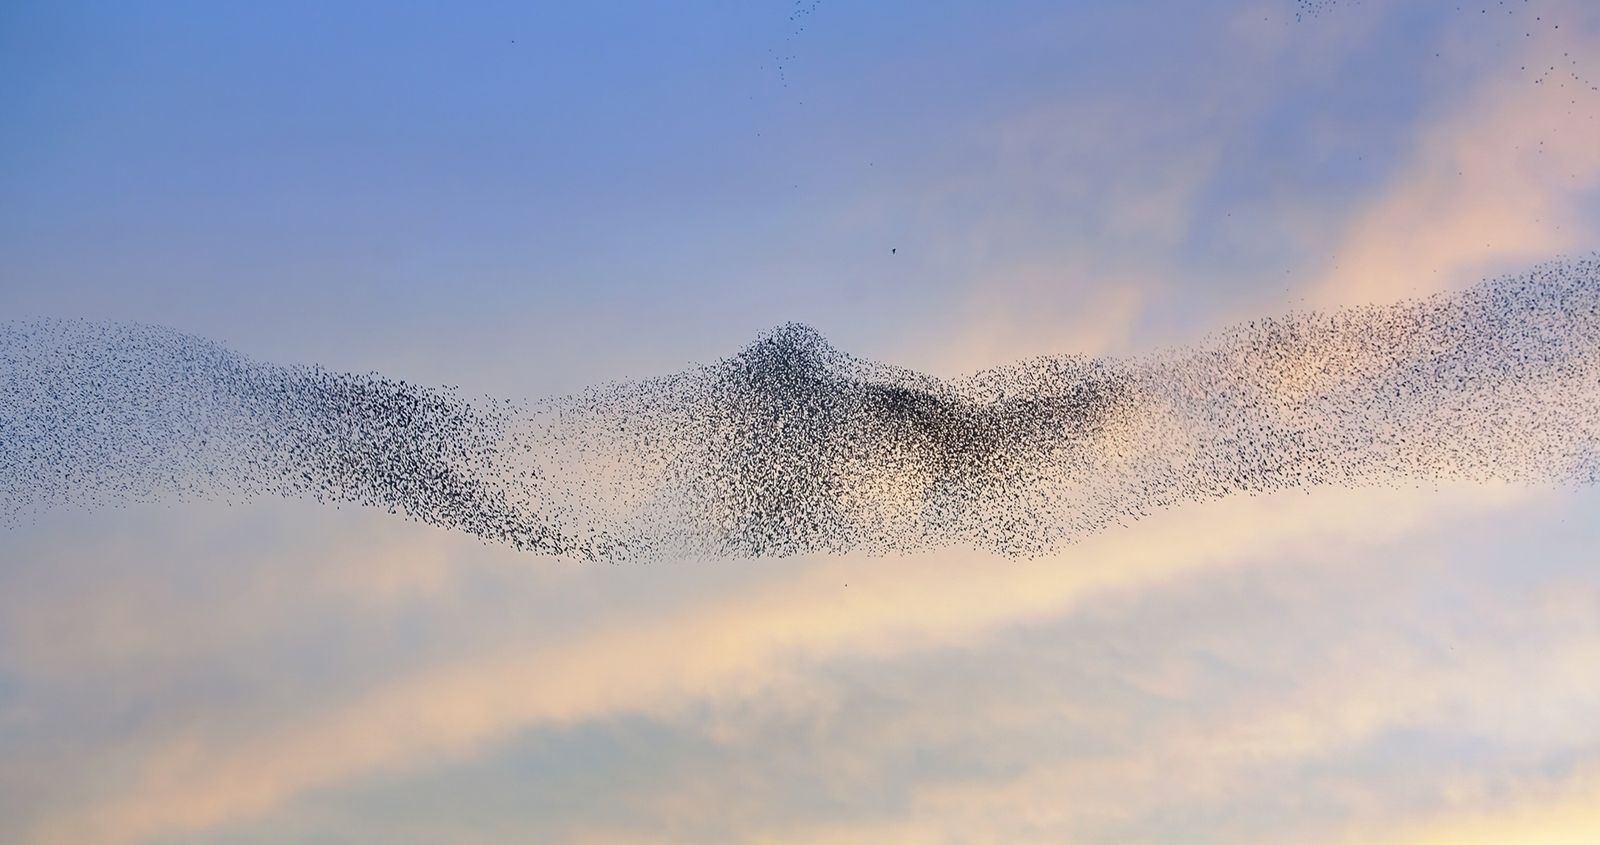
\includegraphics[height=0.62\textheight,keepaspectratio]{stara2.jpg}
    \end{column}
    \begin{column}{0.43\textwidth}
      \begin{itemize}
        \item Bandadas, cardúmenes, colonias bacterianas.
        \item Cada individuo decide sólo con sus vecinos.
        \item Del comportamiento local emerge orden global.
        \item \textbf{Materia activa:} la energía entra localmente, en cada agente.
      \end{itemize}
    \end{column}
  \end{columns}
\end{frame}

% ---------------------------------------------------------------- 4
\begin{frame}{Modelo matemático}
  \textbf{Vicsek (1995)} --- cada partícula adopta la dirección \emph{promedio} de sus vecinos:
  \[
    \theta_i(t+\Delta t) \;=\; \langle \theta(t)\rangle_{r_c} + \Delta\theta_i ,
    \qquad
    \langle\theta\rangle_{r_c} = \arctan\!\frac{\langle\sin\theta\rangle_{r_c}}{\langle\cos\theta\rangle_{r_c}}
  \]

  \textbf{Votante} --- cada partícula \emph{copia} a un vecino elegido al azar:
  \[
    \theta_i(t+\Delta t) \;=\; \theta_{j}(t) + \Delta\theta_i ,
    \qquad j \sim \mathcal{U}\{\,\text{vecinos de } i\,\}
  \]

  \textbf{Posición} --- común a ambos, rapidez constante:
  \[
    \vect{x}_i(t+\Delta t) = \vect{x}_i(t) + \vect{v}_i(t)\,\Delta t ,
    \qquad |\vect{v}_i| = v
  \]

  \vspace{0.3em}
  \centering
  Ruido angular uniforme: $\Delta\theta_i \in [-\eta/2,\; \eta/2]$

  \vspace{0.3em}
  {\footnotesize $\Delta t$, $v$ y $\eta$ son adimensionales (sin unidades físicas asociadas).}
\end{frame}

% =====================================================================
\section{Implementación}
% =====================================================================

% ---------------------------------------------------------------- 6
\begin{frame}{Arquitectura del motor}
  \begin{columns}[c]
    \begin{column}{0.60\textwidth}
      \centering
      \begin{tikzpicture}[
          scale=0.9, transform shape,
          font=\scriptsize,
          box/.style={draw=black!55, rounded corners=2pt, align=center,
                      inner xsep=6pt, inner ysep=5pt, text width=3.4cm},
          est/.style={box, fill=black!10},
          proc/.style={box, fill=white},
          dat/.style={box, fill=black!16},
          fl/.style={-{Latex[length=2mm]}, draw=black!60, thick}
        ]
        \node[est] (sim) {\texttt{Simulation}\\{\tiny estado: \texttt{particles\_}, \texttt{grid\_}, \texttt{rng\_}}};
        \node[proc, below=0.45cm of sim] (grid) {\texttt{Grid::rebuild()}\\{\tiny Cell Index Method}};
        \node[dat,  below=0.4cm of grid] (nl)  {\texttt{NeighborList}};
        \node[proc, below=0.4cm of nl] (rule) {\texttt{circularMeanHeading()}\\ \texttt{voterHeading()}\\{\tiny + \texttt{addAngularNoise()}}};
        \node[proc, below=0.4cm of rule] (int) {integración\\{\tiny posición + condiciones periódicas}};
        \draw[fl] (sim) -- (grid);
        \draw[fl] (grid) -- (nl);
        \draw[fl] (nl) -- (rule);
        \draw[fl] (rule) -- (int);
        \draw[fl] (int.east) -- ++(0.9,0) |- (sim.east);
      \end{tikzpicture}
    \end{column}
    \begin{column}{0.38\textwidth}
      \begin{itemize}
        \item Motor en \textbf{C\texttt{++}20}, sin dependencias externas.
        \item \texttt{Particle} guarda sólo $x$, $y$, $\theta$: la velocidad se deriva de $\theta$.
        \item Los dos modelos comparten todo salvo la regla de alineamiento.
      \end{itemize}
    \end{column}
  \end{columns}
\end{frame}

% ---------------------------------------------------------------- 7
\begin{frame}{Paso temporal: actualización sincrónica}
  \centering
  \begin{tikzpicture}[
      font=\small,
      node distance=0.55cm,
      pas/.style={draw=black!55, rounded corners=2pt, fill=black!5,
                  align=center, inner xsep=8pt, inner ysep=6pt, text width=3.2cm},
      fl/.style={-{Latex[length=2.4mm]}, draw=black!65, very thick}
    ]
    \node[pas] (p1) {\textbf{1. Vecinos}\\[2pt]{\scriptsize reconstruir la grilla desde las posiciones de $t$}};
    \node[pas, right=1.0cm of p1] (p2) {\textbf{2. Ángulos}\\[2pt]{\scriptsize calcular $\theta_i(t{+}\Delta t)$ leyendo \emph{sólo} el estado en $t$}};
    \node[pas, right=1.0cm of p2] (p3) {\textbf{3. Mover}\\[2pt]{\scriptsize avanzar con $\vect{v}_i(t)$ y recién ahí escribir $\theta_i(t{+}\Delta t)$}};
    \draw[fl] (p1) -- (p2);
    \draw[fl] (p2) -- (p3);
  \end{tikzpicture}

  \vspace{1.2em}
  \begin{itemize}
    \item Doble buffer en el paso 2: ninguna partícula ve el ángulo nuevo de otra dentro del mismo paso.
    \item Sin esa separación, el resultado dependería del orden de recorrido.
  \end{itemize}
\end{frame}

% =====================================================================
\section{Simulaciones}
% =====================================================================

% ---------------------------------------------------------------- 9
\begin{frame}{Sistema simulado}
  \begin{columns}[c]
    \begin{column}{0.44\textwidth}
      \centering
      \begin{tikzpicture}[scale=0.85, font=\scriptsize]
        \draw[black!70, thick] (0,0) rectangle (4.4,4.4);
        \foreach \x/\y/\a in {0.8/3.4/20, 1.4/3.0/35, 1.0/2.6/10,
                              3.3/1.2/200, 3.7/1.7/215, 3.0/0.7/190,
                              2.2/2.2/95, 0.6/1.0/300, 3.9/3.6/140}{
          \filldraw[black] (\x,\y) circle (1.4pt);
          \draw[-{Latex[length=1.6mm]}, thick] (\x,\y) -- ++(\a:0.55);
        }
        \draw[dashed, black!60] (2.2,2.2) circle (0.62);
        \node[black!60] at (2.95,2.75) {$r_c$};
        \draw[-{Latex[length=1.6mm]}, gray] (4.4,2.0) -- ++(0.45,0);
        \draw[-{Latex[length=1.6mm]}, gray] (-0.45,2.0) -- ++(0.45,0);
        \node[gray] at (2.2,-0.4) {condiciones periódicas de contorno};
        \draw[<->] (0,4.75) -- node[above] {$L = 10$} (4.4,4.75);
      \end{tikzpicture}
    \end{column}
    \begin{column}{0.54\textwidth}
      \params{
      \textbf{Parámetros fijos}\\[3pt]
      $L = 10$ \quad $r_c = 1$ \quad $\Delta t = 1$\\
      $v = 3\times10^{-2}$\\
      Condiciones periódicas de contorno.\\[8pt]
      \textbf{Input}\\[3pt]
      Ruido $\eta \in [0,\; 2\pi]$\\[8pt]
      \textbf{Densidades} \quad ($N = \rho L^2$)\\[3pt]
      $\rho \in [\,1/3\pi,\; 8\,]$ \quad ($N = 11$ a $800$)
      }
    \end{column}
  \end{columns}
\end{frame}

% ---------------------------------------------------------------- 10
\begin{frame}{Observables}
  \textbf{Polarización} --- módulo de la velocidad media, normalizado:
  \[
    v_a(t) \;=\; \frac{1}{N\,v}\;\Bigg|\sum_{k=1}^{N} \vect{v}_k(t)\Bigg|
    \;\in\; [0,\,1]
  \]

  \textbf{Fracción de la componente gigante} --- sobre el grafo de vecinos dentro de $r_c$:
  \[
    S(t) \;=\; \frac{N_{\max}(t)}{N},
    \qquad N_{\max} = \text{tamaño del cluster más grande}
  \]

  \vspace{0.4em}
  \hrule
  \vspace{0.5em}

  \params{
  Escalar reportado: media temporal en el estacionario.\\[3pt]
  Realizaciones: 10.\\[3pt]
  Pasos: $2\times10^{3}$ ($\rho = 2,\,4,\,8$), \; $1\times10^{4}$ ($\rho < 1$).\\[3pt]
  Ventana de promedio: desde el inicio del estacionario, medido por ruido.
  }
\end{frame}

% =====================================================================
\section{Resultados}
% =====================================================================

% ---------------------------------------------------------------- 12
\begin{frame}{Vicsek: dinámica característica}
  \begin{columns}[T]
    \begin{column}{0.36\textwidth}
      \animacion{frame_vicsek_rho2_ordenado.png}{1{,}0}{https://youtu.be/PENDIENTE-1}
    \end{column}
    \begin{column}{0.36\textwidth}
      \animacion{frame_vicsek_rho2_desordenado.png}{4{,}0}{https://youtu.be/PENDIENTE-2}
    \end{column}
    \begin{column}{0.26\textwidth}
      \params{$\rho = 2$ \ ($N = 200$)\\[6pt]Color según el ángulo de la velocidad.}
    \end{column}
  \end{columns}
\end{frame}

% ---------------------------------------------------------------- 13
\begin{frame}{Vicsek: evolución temporal de la polarización}
  \begin{columns}[c]
    \begin{column}{0.72\textwidth}
      \centering\includegraphics[width=0.98\linewidth,height=0.75\textheight,keepaspectratio]{va_t_vicsek_rho2.png}
    \end{column}
    \begin{column}{0.26\textwidth}
      \params{$\rho = 2$ \ ($N = 200$)}
    \end{column}
  \end{columns}
\end{frame}

% ---------------------------------------------------------------- 14
\begin{frame}{Vicsek: polarización en función del ruido}
  \begin{columns}[c]
    \begin{column}{0.72\textwidth}
      \centering\includegraphics[width=0.98\linewidth,height=0.75\textheight,keepaspectratio]{va_eta_vicsek.png}
    \end{column}
    \begin{column}{0.26\textwidth}
      \params{$2\times10^{3}$ pasos\\[6pt]Realizaciones: 10}
    \end{column}
  \end{columns}
\end{frame}

% ---------------------------------------------------------------- 15
\begin{frame}{Vicsek: evolución temporal de la componente gigante}
  \begin{columns}[c]
    \begin{column}{0.72\textwidth}
      \centering\includegraphics[width=0.98\linewidth,height=0.75\textheight,keepaspectratio]{S_t_vicsek_rho1_pi.png}
    \end{column}
    \begin{column}{0.26\textwidth}
      \params{$\rho = 1/\pi$ \ ($N = 32$)}
    \end{column}
  \end{columns}
\end{frame}

% ---------------------------------------------------------------- 16
\begin{frame}{Vicsek: componente gigante en función del ruido}
  \begin{columns}[c]
    \begin{column}{0.72\textwidth}
      \centering\includegraphics[width=0.98\linewidth,height=0.75\textheight,keepaspectratio]{S_eta_vicsek.png}
    \end{column}
    \begin{column}{0.26\textwidth}
      \params{$2\times10^{3}$ pasos ($\rho \geq 2$)\\$1\times10^{4}$ pasos ($\rho < 1$)\\[6pt]Realizaciones: 10}
    \end{column}
  \end{columns}
\end{frame}

% ---------------------------------------------------------------- 17
\begin{frame}{Votante: dinámica característica}
  \begin{columns}[T]
    \begin{column}{0.36\textwidth}
      \animacion{frame_voter_rho2_ordenado.png}{0{,}05}{https://youtu.be/PENDIENTE-3}
    \end{column}
    \begin{column}{0.36\textwidth}
      \animacion{frame_voter_rho2_desordenado.png}{1{,}0}{https://youtu.be/PENDIENTE-4}
    \end{column}
    \begin{column}{0.26\textwidth}
      \params{$\rho = 2$ \ ($N = 200$)\\[6pt]Color según el ángulo de la velocidad.}
    \end{column}
  \end{columns}
\end{frame}

% ---------------------------------------------------------------- 18
\begin{frame}{Votante: evolución temporal de la polarización}
  \begin{columns}[c]
    \begin{column}{0.72\textwidth}
      \centering\includegraphics[width=0.98\linewidth,height=0.75\textheight,keepaspectratio]{va_t_voter_rho2.png}
    \end{column}
    \begin{column}{0.26\textwidth}
      \params{$\rho = 2$ \ ($N = 200$)}
    \end{column}
  \end{columns}
\end{frame}

% ---------------------------------------------------------------- 19
\begin{frame}{Votante: polarización en función del ruido}
  \begin{columns}[c]
    \begin{column}{0.72\textwidth}
      \centering\includegraphics[width=0.98\linewidth,height=0.75\textheight,keepaspectratio]{va_eta_voter.png}
    \end{column}
    \begin{column}{0.26\textwidth}
      \params{$2\times10^{3}$ pasos\\[6pt]Realizaciones: 10}
    \end{column}
  \end{columns}
\end{frame}

% ---------------------------------------------------------------- 20
\begin{frame}{Votante: evolución temporal de la componente gigante}
  \begin{columns}[c]
    \begin{column}{0.72\textwidth}
      \centering\includegraphics[width=0.98\linewidth,height=0.75\textheight,keepaspectratio]{S_t_voter_rho1_pi.png}
    \end{column}
    \begin{column}{0.26\textwidth}
      \params{$\rho = 1/\pi$ \ ($N = 32$)}
    \end{column}
  \end{columns}
\end{frame}

% ---------------------------------------------------------------- 21
\begin{frame}{Votante: componente gigante en función del ruido}
  \begin{columns}[c]
    \begin{column}{0.72\textwidth}
      \centering\includegraphics[width=0.98\linewidth,height=0.75\textheight,keepaspectratio]{S_eta_voter.png}
    \end{column}
    \begin{column}{0.26\textwidth}
      \params{$2\times10^{3}$ pasos ($\rho \geq 2$)\\$1\times10^{4}$ pasos ($\rho < 1$)\\[6pt]Realizaciones: 10}
    \end{column}
  \end{columns}
\end{frame}

% ---------------------------------------------------------------- 22
\begin{frame}{Comparación: polarización}
  \begin{columns}[c]
    \begin{column}{0.72\textwidth}
      \centering\includegraphics[width=0.98\linewidth,height=0.75\textheight,keepaspectratio]{va_eta_comparacion_medias.png}
    \end{column}
    \begin{column}{0.26\textwidth}
      \params{Sólo el promedio\\[6pt]Realizaciones: 10}
    \end{column}
  \end{columns}
\end{frame}

% ---------------------------------------------------------------- 23
\begin{frame}{Comparación: componente gigante}
  \begin{columns}[c]
    \begin{column}{0.72\textwidth}
      \centering\includegraphics[width=0.98\linewidth,height=0.75\textheight,keepaspectratio]{S_eta_comparacion_sub_medias.png}
    \end{column}
    \begin{column}{0.26\textwidth}
      \params{$\rho = 1/\pi,\ 1/2\pi,\ 1/3\pi$\\$1\times10^{4}$ pasos\\[6pt]A $\rho = 2,\,4,\,8$ resulta $S \approx 1$ para todo $\eta$ en ambos modelos.}
    \end{column}
  \end{columns}
\end{frame}

% ---------------------------------------------------------------- 24
\begin{frame}{Polarización en función de la componente gigante}
  \begin{columns}[c]
    \begin{column}{0.84\textwidth}
      \centering\includegraphics[width=0.99\linewidth,height=0.66\textheight,keepaspectratio]{va_vs_S_paneles.png}
    \end{column}
    \begin{column}{0.15\textwidth}
      \params{Cada punto es un valor de $\eta$.}
    \end{column}
  \end{columns}
\end{frame}

% ---------------------------------------------------------------- 25
\begin{frame}{Tiempo de ejecución del Cell Index Method}
  \begin{columns}[c]
    \begin{column}{0.72\textwidth}
      \centering\includegraphics[width=0.98\linewidth,height=0.75\textheight,keepaspectratio]{benchmark_tp1_vs_tp2.png}
    \end{column}
    \begin{column}{0.26\textwidth}
      \params{
      $L = 10$, \ $r_c = 1$, \ $M = 9$\\
      Partículas puntuales\\[6pt]
      TP2: una medición por paso, $2\times10^{3}$ pasos\\[4pt]
      TP1: búsqueda aislada, repetida $2\times10^{2}$ veces
      }
    \end{column}
  \end{columns}
\end{frame}

% =====================================================================
\section{Conclusiones}
% =====================================================================

% ---------------------------------------------------------------- 27
\begin{frame}{Conclusiones}
  \begin{itemize}
    \item En ambos modelos $v_a$ decrece monótonamente con el ruido: hay transición de orden a desorden.
    \vspace{0.4em}
    \item En Vicsek el ruido tolerado \textbf{crece} con la densidad ($v_a = 0{,}5$ en $\eta = 2{,}9$, $3{,}2$ y $3{,}4$ para $\rho = 2$, $4$ y $8$).
    \vspace{0.4em}
    \item En el votante la dependencia se \textbf{invierte} ($\eta = 0{,}34$, $0{,}26$ y $0{,}21$) y la región ordenada es un orden de magnitud más angosta.
    \vspace{0.4em}
    \item $S \approx 1$ para $\rho = 2,\,4,\,8$ en todo el rango de $\eta$: la componente gigante sólo distingue regímenes en las densidades subcríticas.
    \vspace{0.4em}
    \item El CIM medido dentro del paso temporal tiene el mismo escalado con $N$ que medido aisladamente en el TP1.
  \end{itemize}
\end{frame}

% ---------------------------------------------------------------- 28
\begin{frame}[plain]
  \vfill
  \begin{beamercolorbox}[sep=8pt,center]{title}
    \usebeamerfont{title} Muchas gracias
  \end{beamercolorbox}
  \vfill
\end{frame}

\end{document}
